\chapter{Complete Empirical Telemetry Catalogue}
\label{chap:telemetry_catalogue}

This appendix provides an exhaustive, multi-panel telemetry record across all evaluated GLUE sequence classification benchmarks on \texttt{roberta-base}, covering both homogeneous consensus regimes (Dirichlet concentration parameter $\alpha = 1000.0$) and severe statistical heterogeneity regimes ($\alpha = 0.5$) across small ($C = 20$) and scaled ($C = 50$) client cohorts.

Each multi-panel figure provides six simultaneous optimization diagnostic views:
\begin{enumerate}
    \item \textbf{Panel (a) --- Validation Accuracy vs. Rounds}: Evaluates convergence rate, peak generalization milestones, and post-peak trajectory stability.
    \item \textbf{Panel (b) --- Accuracy vs. Total Network Communication}: Plots validation accuracy directly against cumulative bi-directional Float32 network communication ($\text{Total MB}$), evaluating bandwidth efficiency.
    \item \textbf{Panel (c) --- Realized Local Epochs per Round ($\bar{e}$)}: Tracks dynamic local epoch allocations governed by closed-loop variance tracking within $[e_{\min}, e_{\max}]$.
    \item \textbf{Panel (d) --- Dual-Track Threshold Dynamics ($\theta_A, \theta_B$)}: Visualizes the decoupled threshold adaptation curves for down-projection factor $A$ and up-projection factor $B$.
    \item \textbf{Panel (e) --- Client Coordinate Drift Variance ($\bar{\nu}$)}: Quantifies instantaneous inter-client parameter variance in active low-rank coordinate space.
    \item \textbf{Panel (f) --- Drift Variance vs. Cumulative Local Epochs}: Diagnoses coordinate dispersion as a function of total on-device computation passes.
\end{enumerate}

\clearpage
\section{Multi-Genre Natural Language Inference (MNLI)}
\label{sec:app_mnli}

\begin{figure}[H]
    \centering
    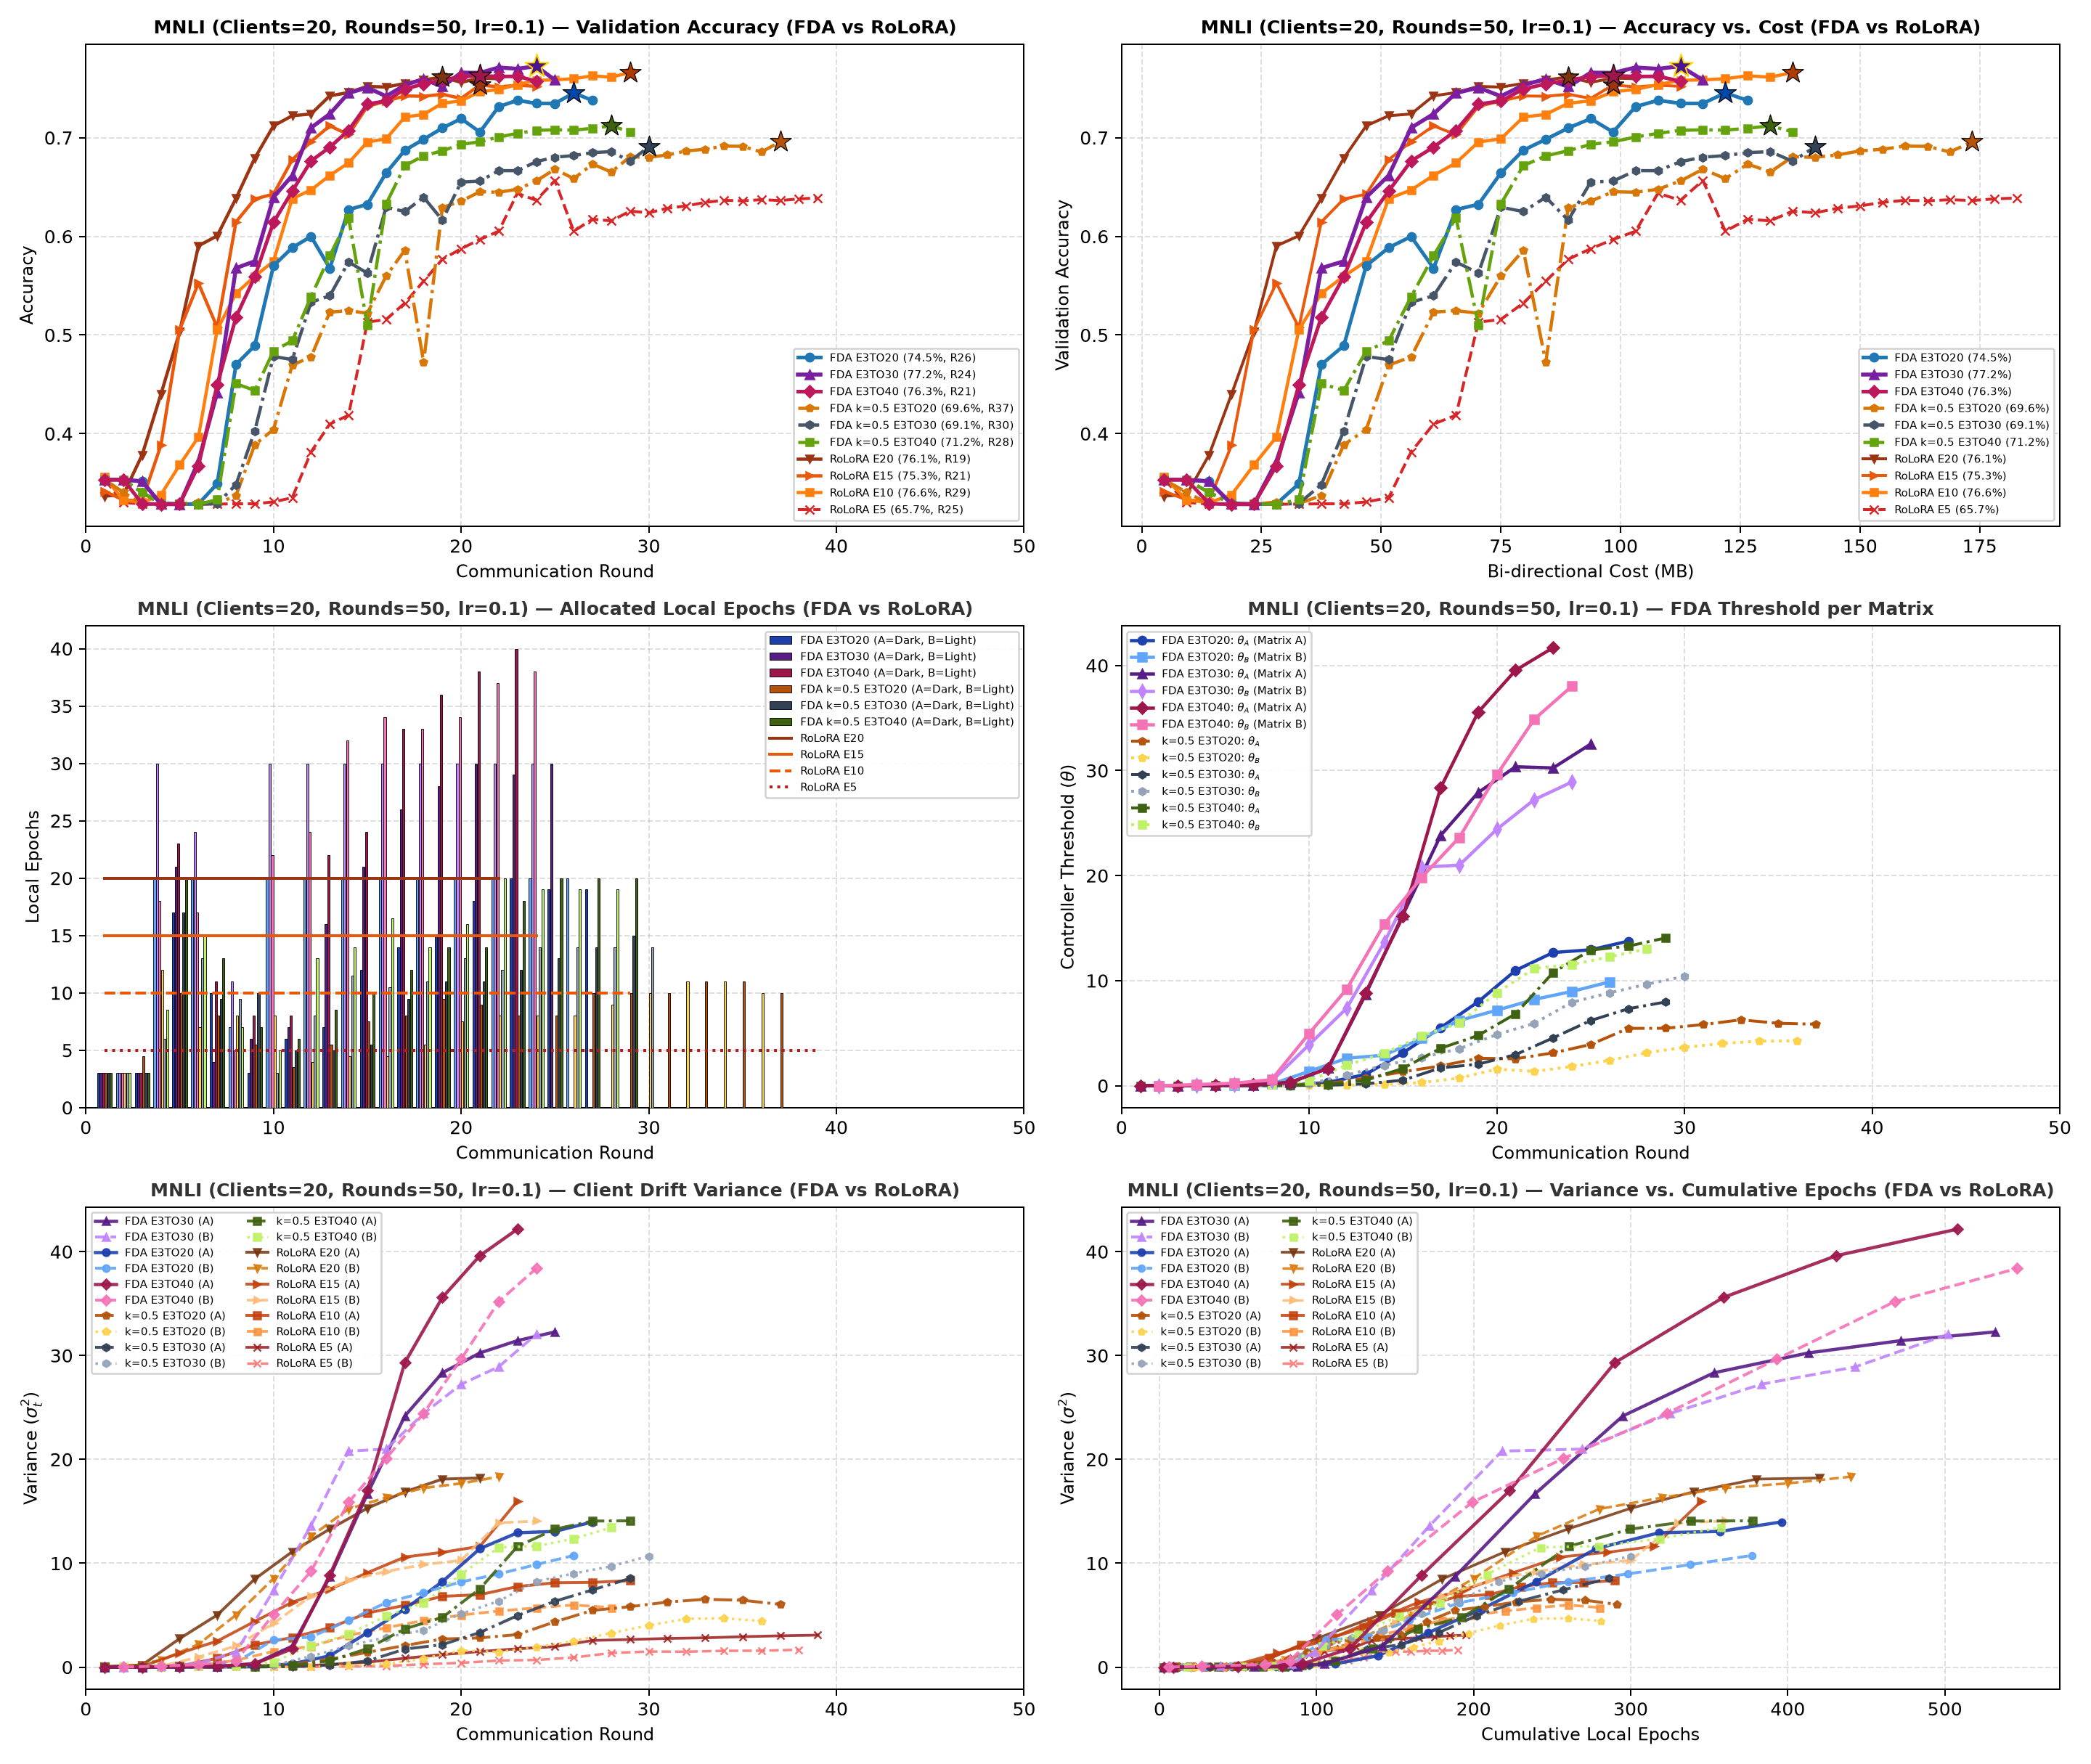
\includegraphics[width=0.62\textwidth]{figures/01_MNLI_C20_R50_LR0.1_all6_telemetry_stacked.png}
    \caption{Multi-panel optimization telemetry on MNLI ($C=20, R_{\max}=50, \eta_c=0.1, \alpha=1000.0$) under homogeneous consensus.}
    \label{fig:app_mnli_c20_iid}
\end{figure}

Figure~\ref{fig:app_mnli_c20_iid} depicts the baseline optimization telemetry on 3-class MNLI with 20 clients in an IID consensus environment:
\begin{itemize}
    \item \textbf{Consensus Trajectories (Panels a \& b)}: All configurations advance steadily toward $76\%$ validation accuracy. FDA-RoLoRA ($k=1.0$) attains $76.28\%$, matching tuned static schedules ($76.02\%$).
    \item \textbf{Controller Epoch Expansion (Panels c \& d)}: In the absence of label conflict, the adaptive controller safely expands local training to $\bar{e} = 13.42$ epochs per round.
    \item \textbf{Bounded Coordinate Drift (Panels e \& f)}: Drift variance remains naturally constrained ($\bar{\nu} \approx 3.71\text{--}6.55$), confirming that homogeneous updates move along aligned consensus gradients.
\end{itemize}

\clearpage
\begin{figure}[H]
    \centering
    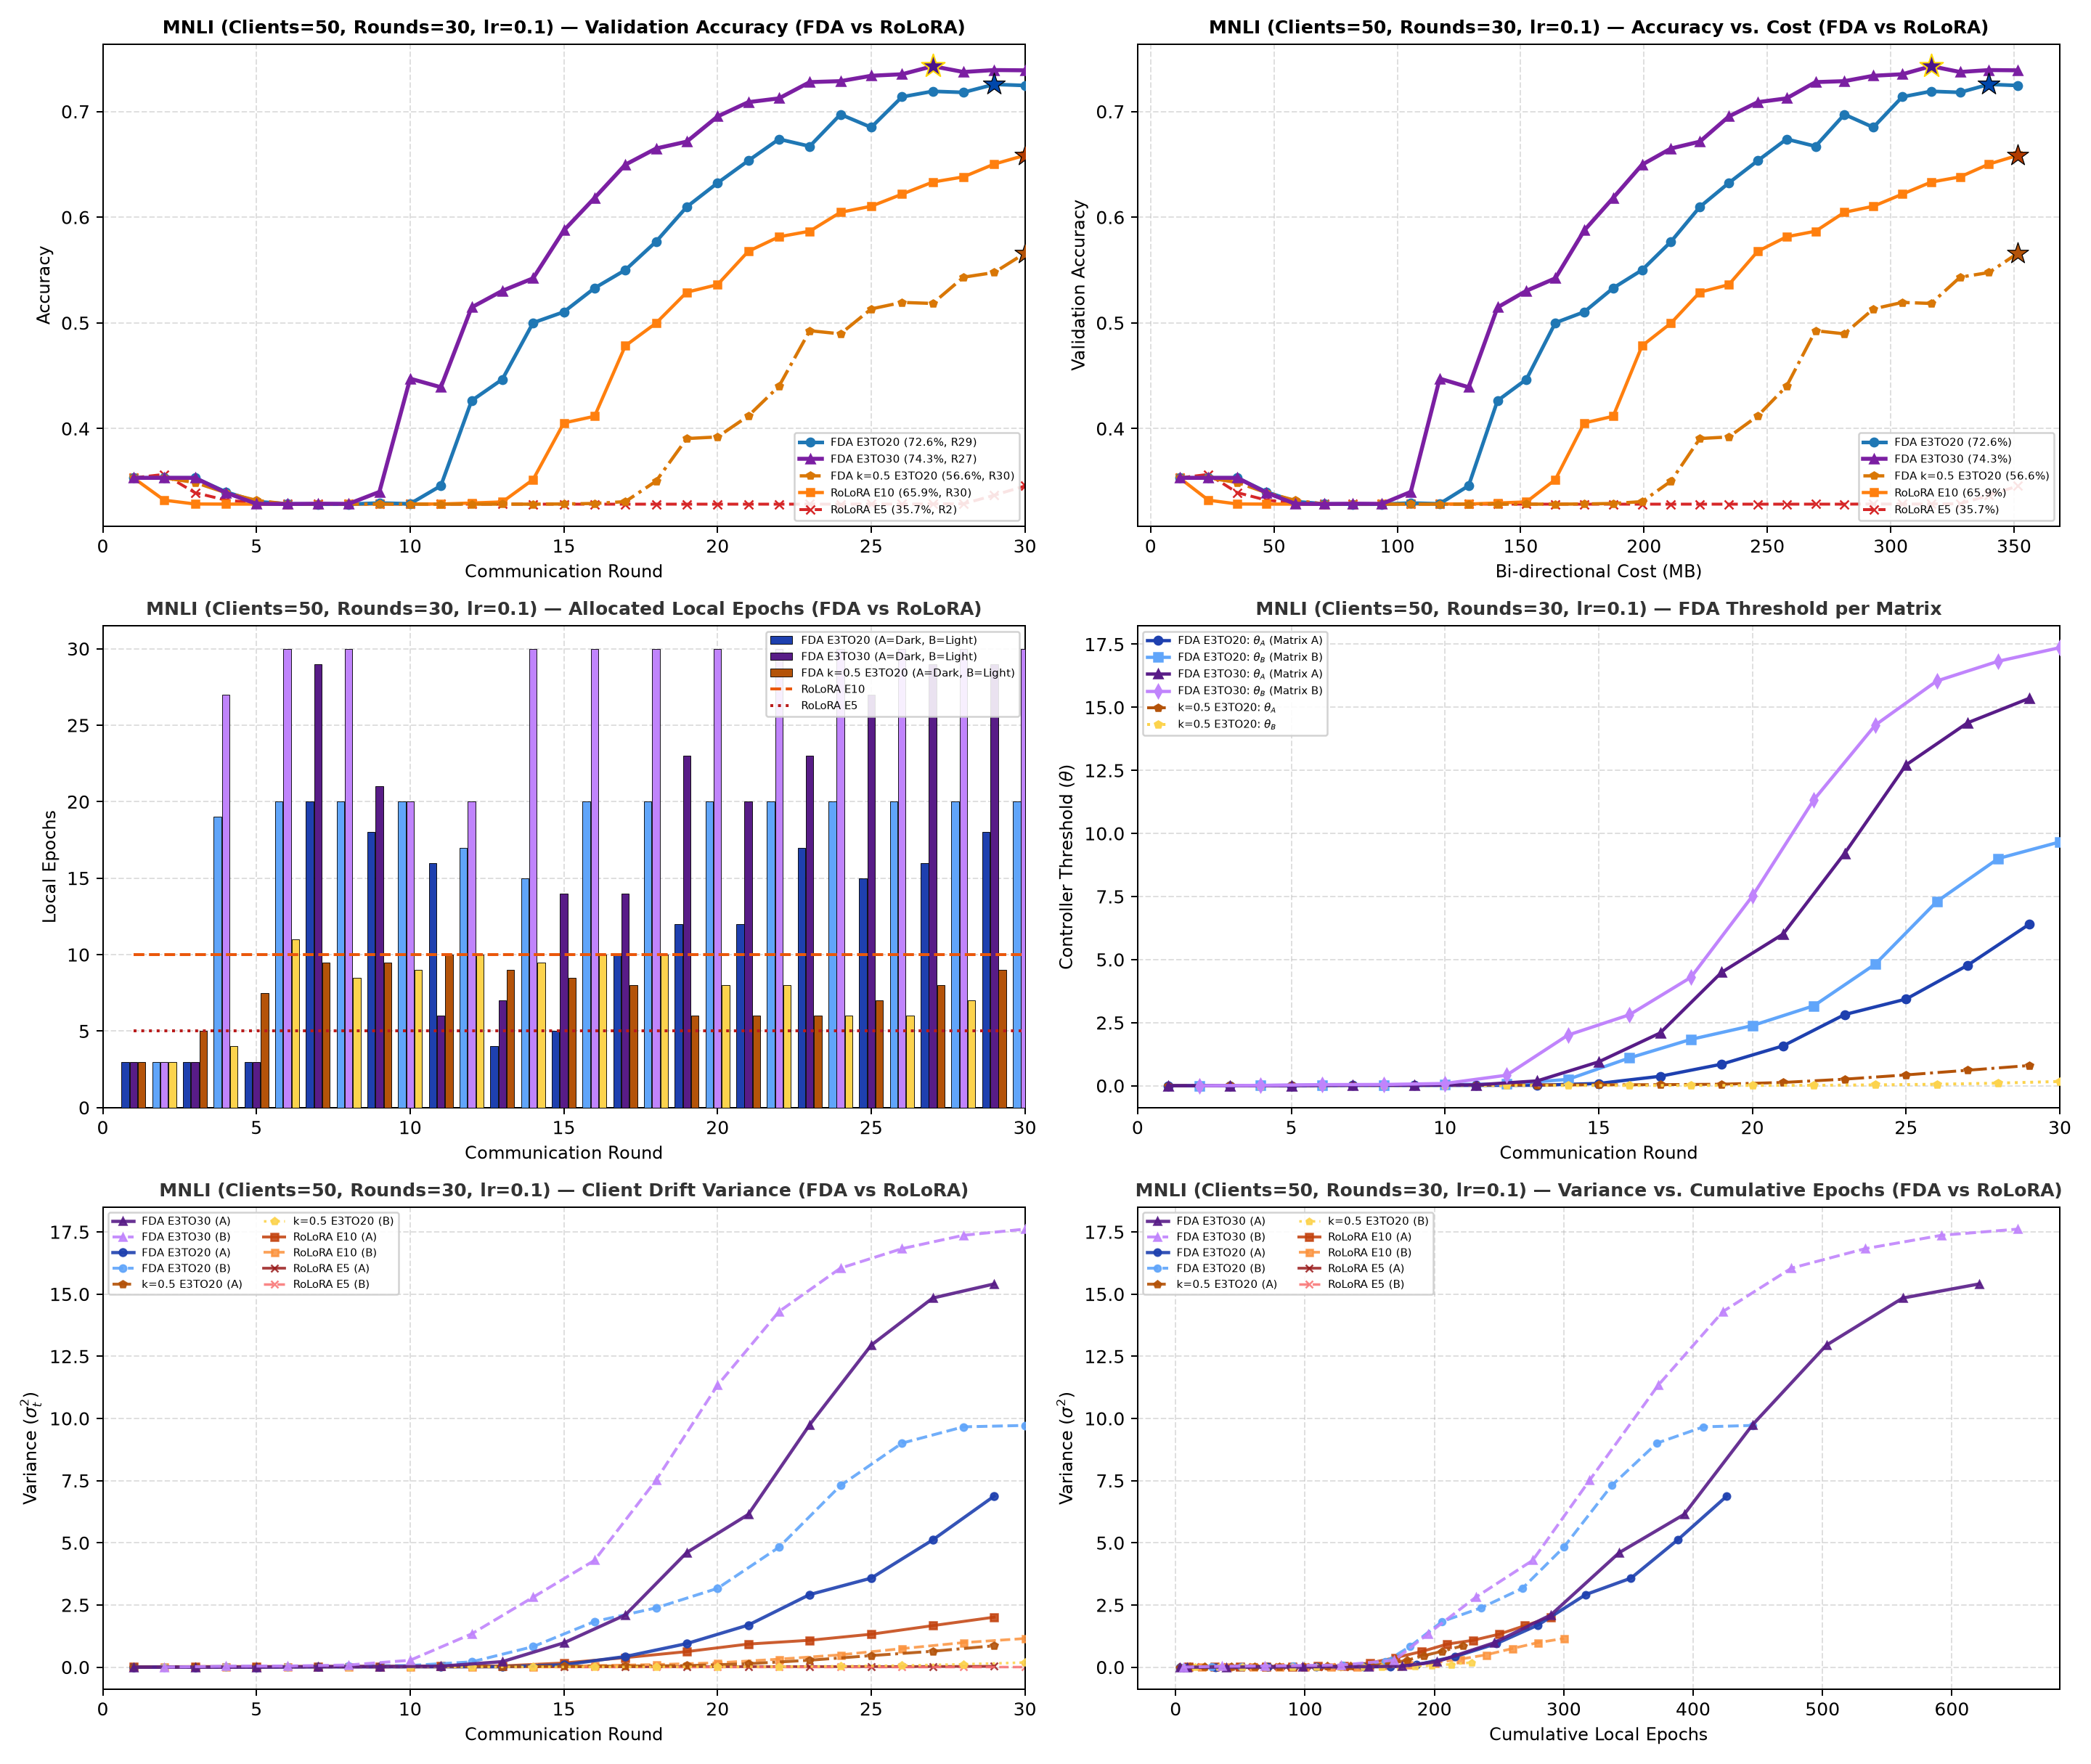
\includegraphics[width=0.62\textwidth]{figures/03_MNLI_C50_R30_LR0.1_all6_telemetry_stacked.png}
    \caption{Multi-panel optimization telemetry on MNLI ($C=50, R_{\max}=30, \eta_c=0.1, \alpha=1000.0$) under cohort scaling.}
    \label{fig:app_mnli_c50_iid}
\end{figure}

Figure~\ref{fig:app_mnli_c50_iid} illustrates optimization dynamics when scaling the client cohort to $C=50$ under homogeneous consensus:
\begin{itemize}
    \item \textbf{Overcoming Stagnation (Panels a \& b)}: Static RoLoRA ($E=10$) plateaus prematurely at $64.93\%$, whereas FDA-RoLoRA ($k=1.0$) continues advancing steadily to $\mathbf{69.08\%}$ ($+4.15\%$).
    \item \textbf{Deep Horizon Scaling (Panels c \& d)}: The controller dynamically expands computational depth to $\bar{e} = 12.15$, extracting greater progress per communication round.
    \item \textbf{Linear Aggregation Stability (Panels e \& f)}: Drift variance stabilizes at $\bar{\nu} = 1.115$, demonstrating that alternating coordinate optimization reliably aggregates 50 clients.
\end{itemize}

\clearpage
\begin{figure}[H]
    \centering
    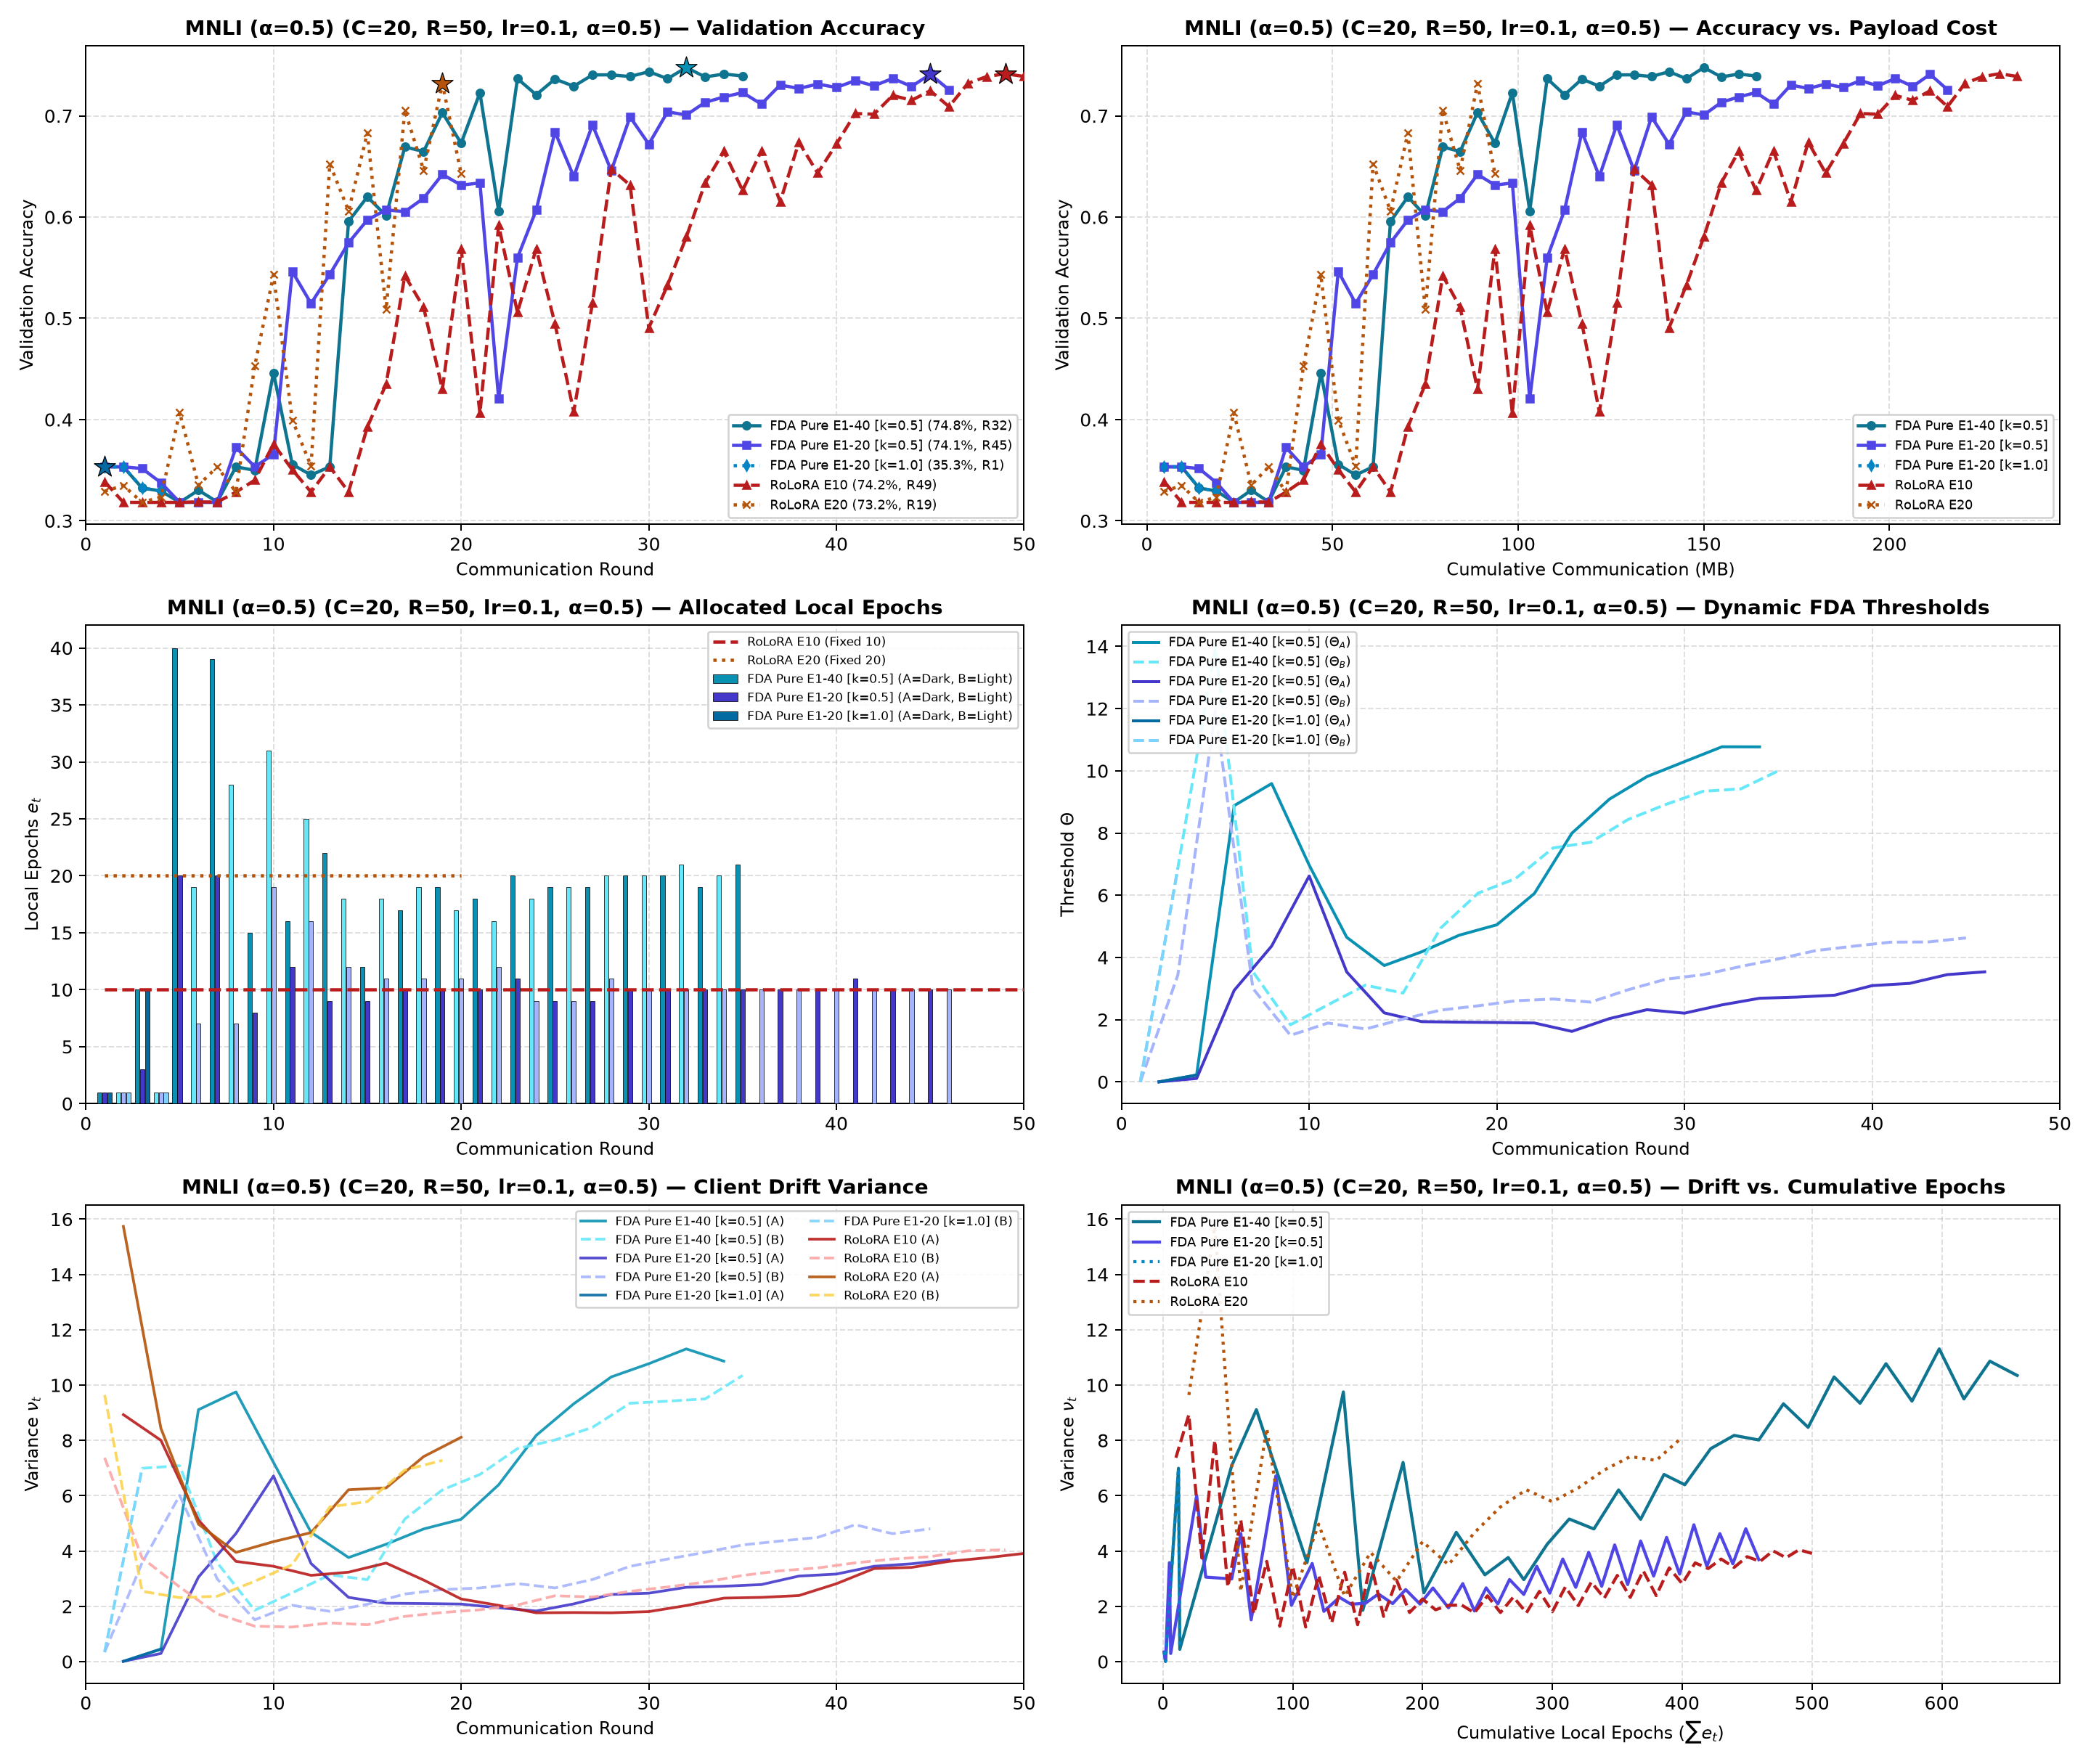
\includegraphics[width=0.62\textwidth]{figures/17_MNLI_C20_R50_LR0.1_A0.5_all6_telemetry_stacked.png}
    \caption{Multi-panel optimization telemetry on MNLI ($C=20, R_{\max}=50, \eta_c=0.1, \alpha=0.5$) under severe Dirichlet label skew.}
    \label{fig:app_mnli_c20_non_iid}
\end{figure}

Figure~\ref{fig:app_mnli_c20_non_iid} displays telemetry on MNLI under acute Dirichlet label skew ($\alpha=0.5$):
\begin{itemize}
    \item \textbf{Post-Peak Collapse of Static Baselines (Panel a)}: Static RoLoRA ($E=20$) peaks at $72.54\%$ at round 17 and then collapses catastrophically to $68.09\%$ due to unconstrained local over-fitting.
    \item \textbf{Dynamic Braking and Stability (Panels c \& d)}: FDA-RoLoRA dynamically truncates local training when coordinate variance expands, safely bounding client trajectories.
    \item \textbf{Acute Variance Surge (Panels e \& f)}: Parameter drift variance surges to peak values of $10.68\text{--}13.73$, verifying the massive orthogonal pulling forces induced by 3-class label imbalance.
\end{itemize}

\clearpage
\section{Question Natural Language Inference (QNLI)}
\label{sec:app_qnli}

\begin{figure}[H]
    \centering
    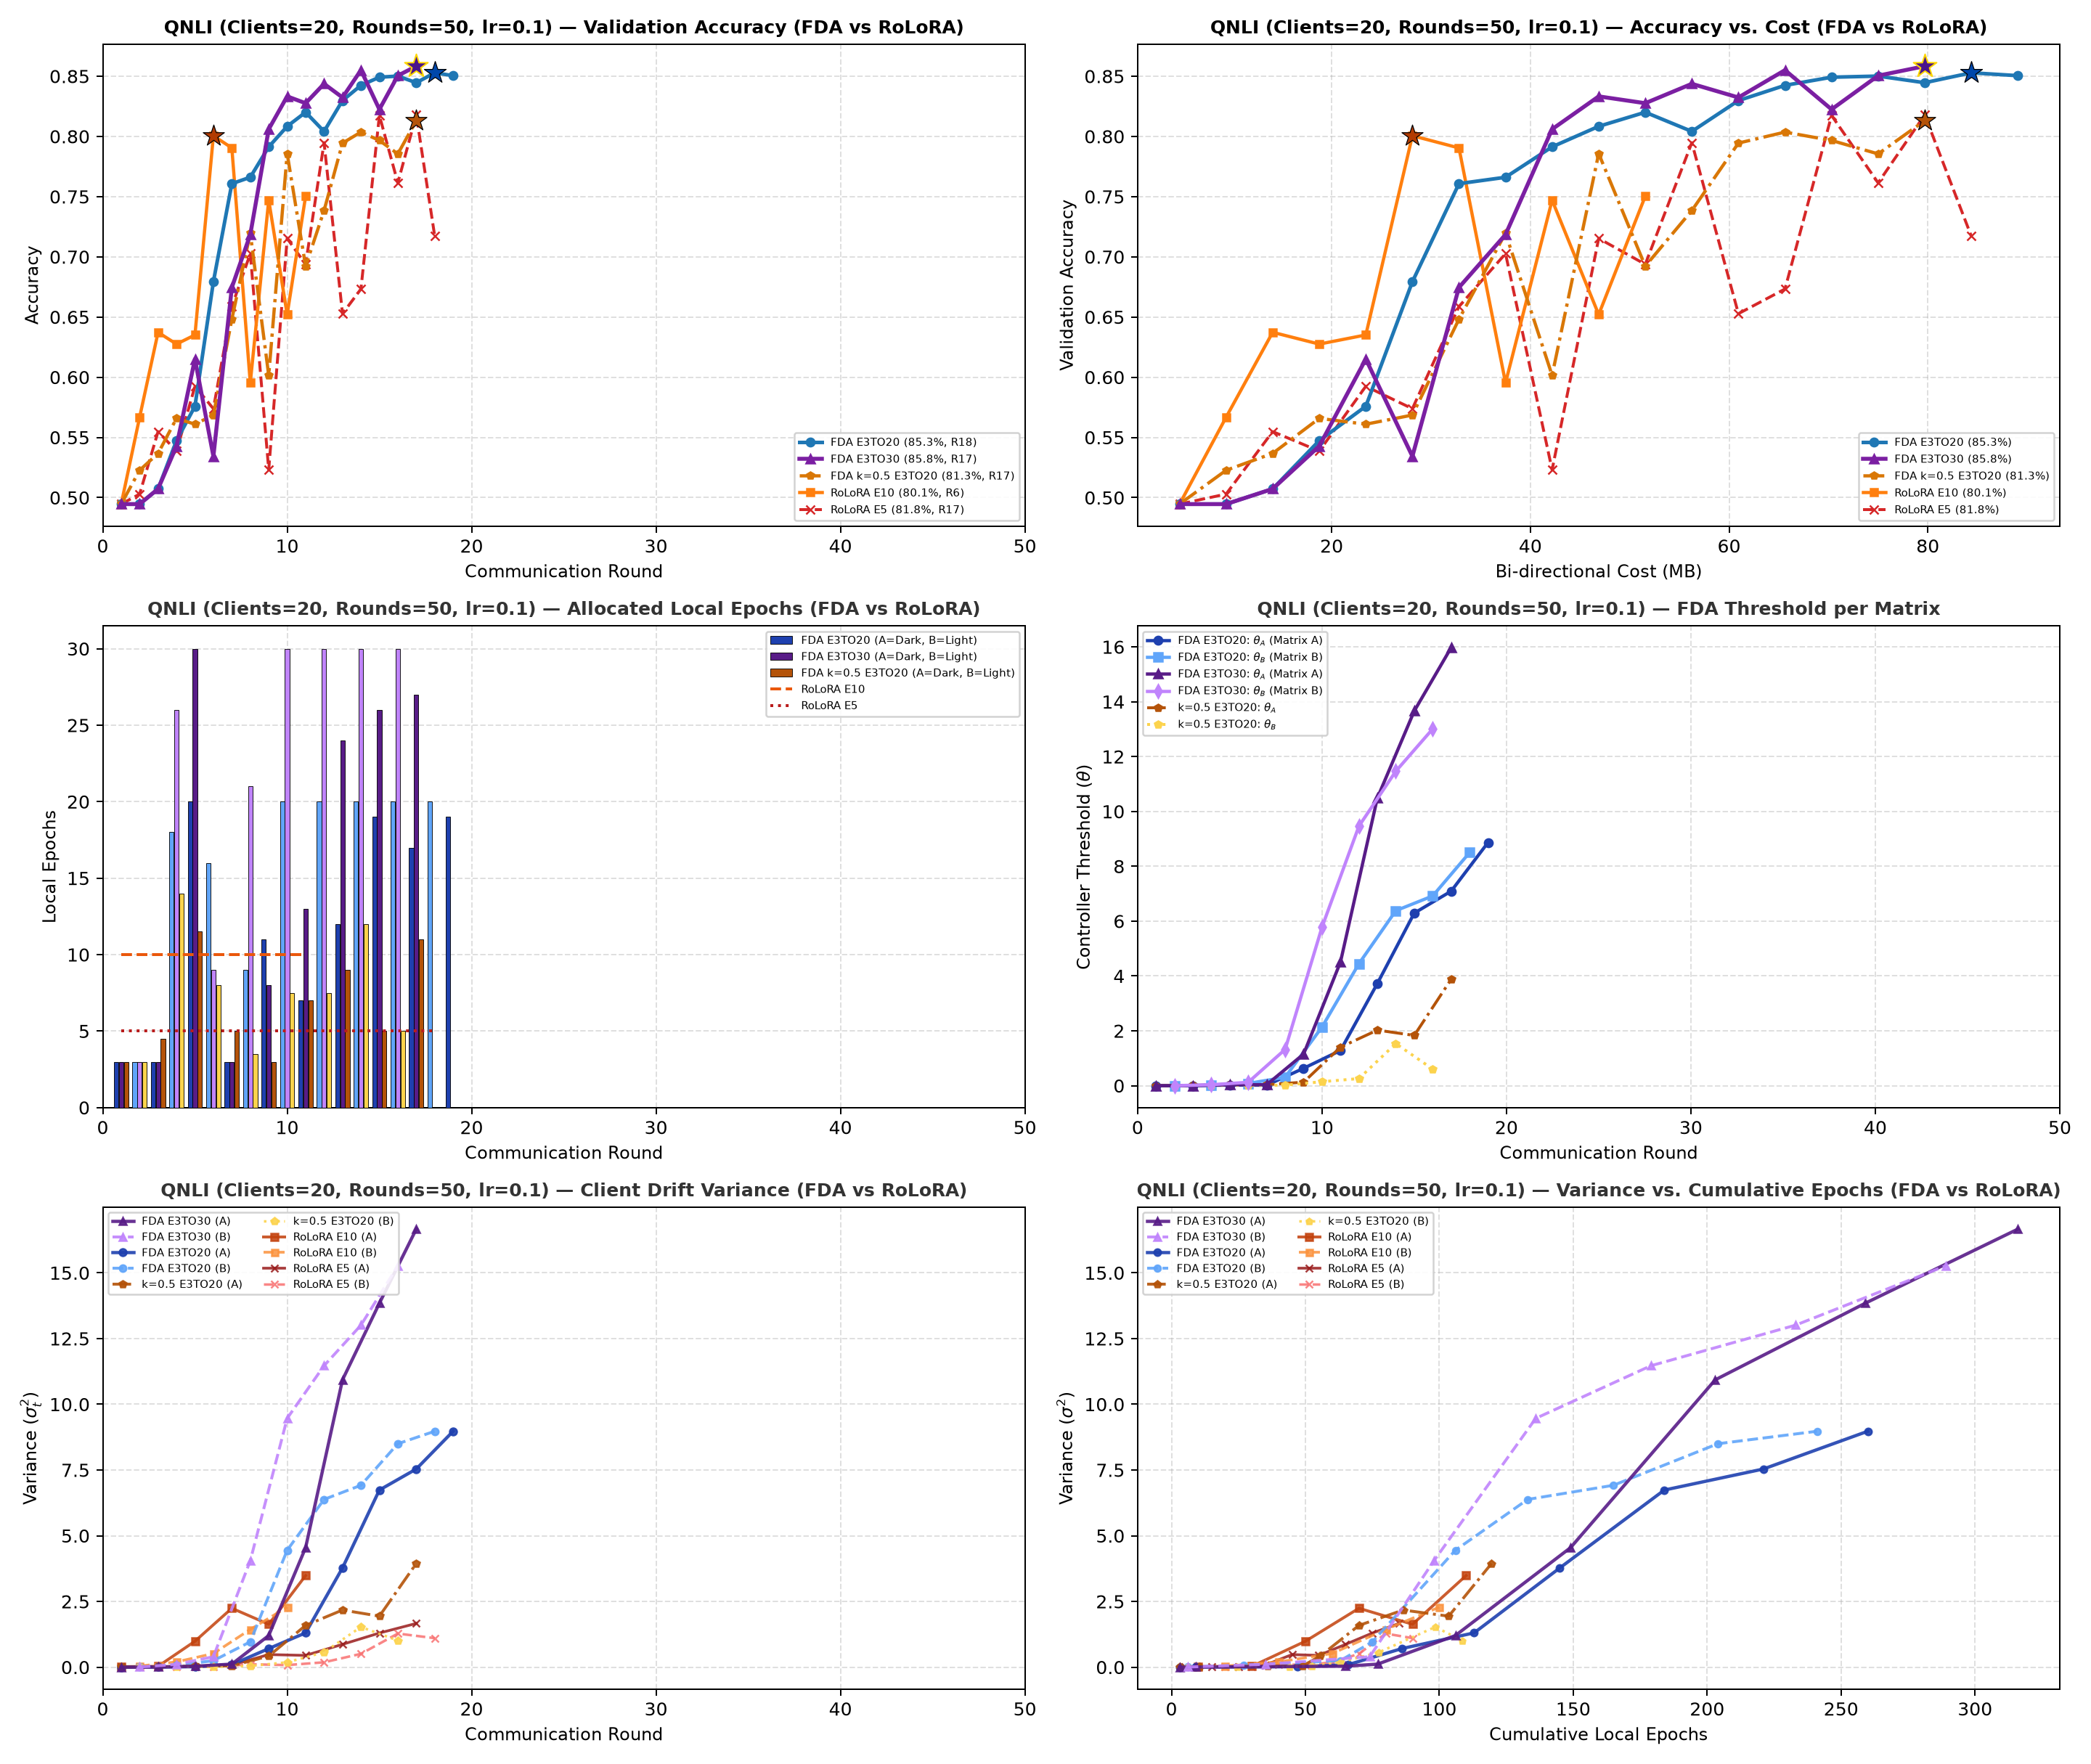
\includegraphics[width=0.62\textwidth]{figures/05_QNLI_C20_R50_LR0.1_all6_telemetry_stacked.png}
    \caption{Multi-panel optimization telemetry on QNLI ($C=20, R_{\max}=50, \eta_c=0.1, \alpha=1000.0$) under homogeneous consensus.}
    \label{fig:app_qnli_c20_iid}
\end{figure}

Figure~\ref{fig:app_qnli_c20_iid} illustrates binary question-answering inference on 20 clients under homogeneous partitioning:
\begin{itemize}
    \item \textbf{Generalization Mastery (Panels a \& b)}: FDA-RoLoRA ($k=1.0$) reaches a peak validation accuracy of $\mathbf{83.14\%}$, outperforming static RoLoRA ($81.83\%$).
    \item \textbf{Smooth Epoch Tracking (Panels c \& d)}: Local computation executes at $\bar{e} = 9.85$ epochs per round, guided by smooth threshold progression.
    \item \textbf{Suppressed Coordinate Variance (Panels e \& f)}: Parameter drift variance remains tightly contained ($\bar{\nu} \approx 1.11$), confirming rapid convergence toward the global consensus trajectory.
\end{itemize}

\clearpage
\begin{figure}[H]
    \centering
    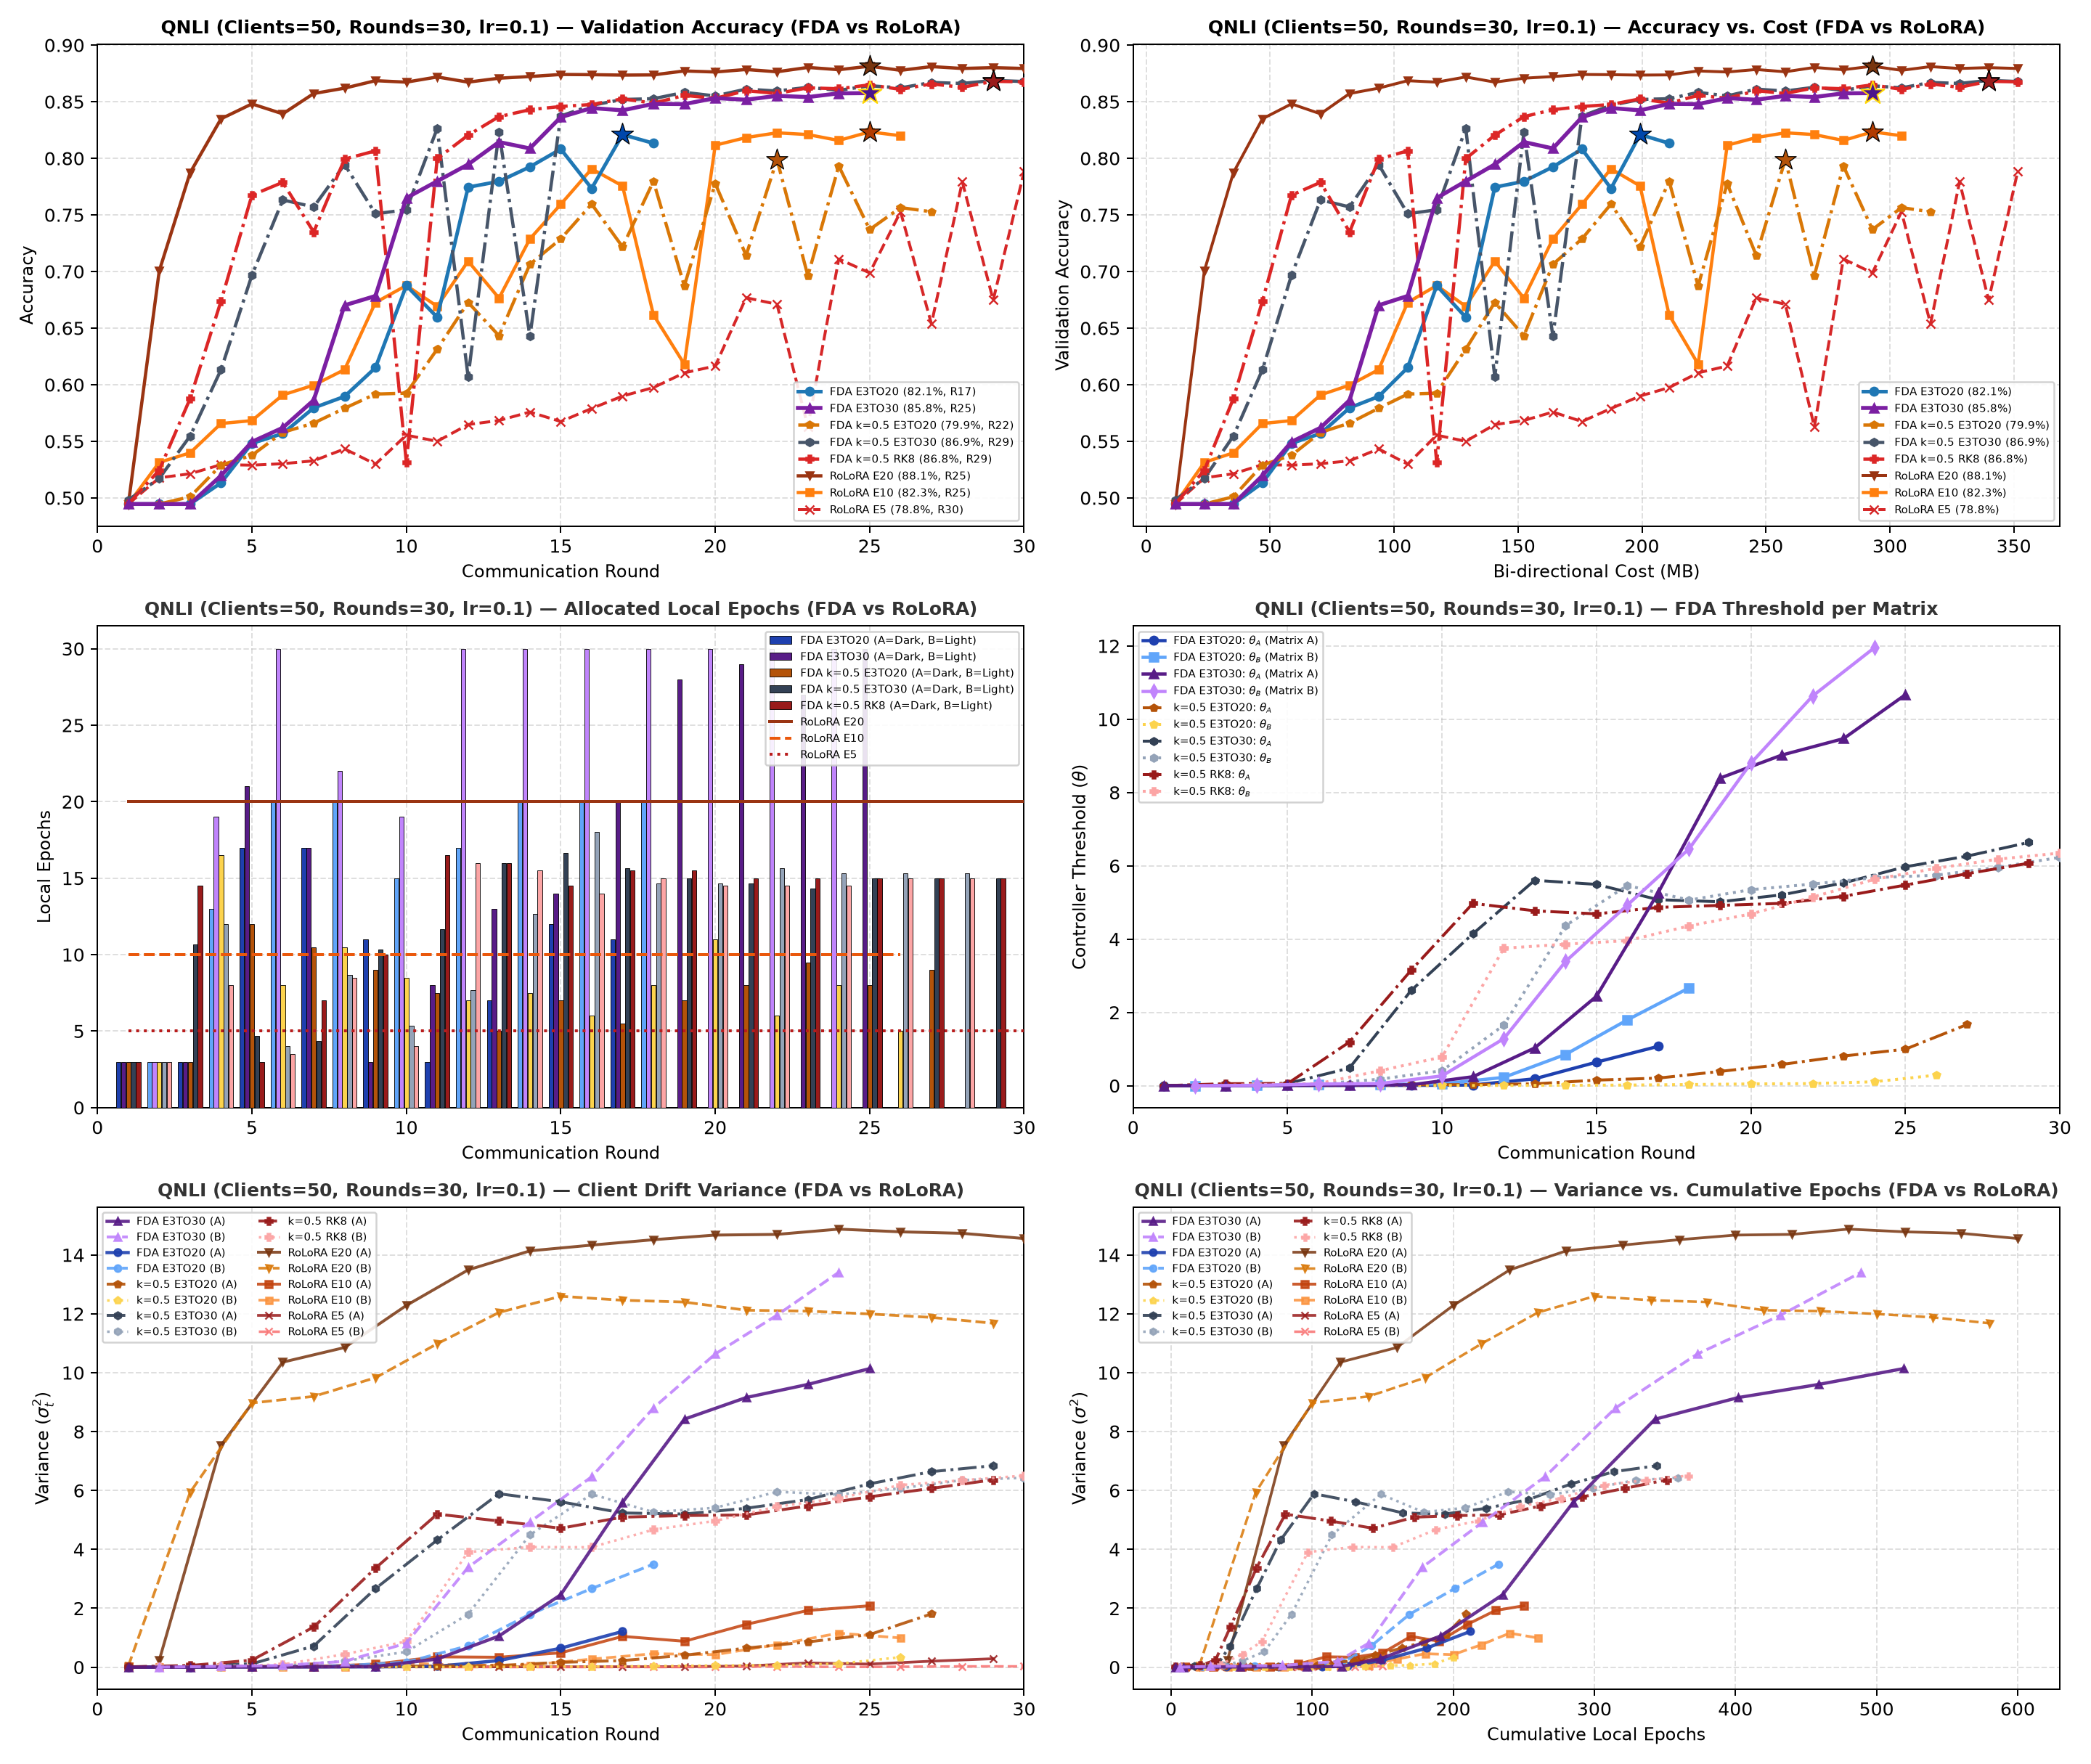
\includegraphics[width=0.62\textwidth]{figures/07_QNLI_C50_R30_LR0.1_all6_telemetry_stacked.png}
    \caption{Multi-panel optimization telemetry on QNLI ($C=50, R_{\max}=30, \eta_c=0.1, \alpha=1000.0$) under cohort scaling.}
    \label{fig:app_qnli_c50_iid}
\end{figure}

Figure~\ref{fig:app_qnli_c50_iid} depicts QNLI telemetry when scaling client participation to $C=50$:
\begin{itemize}
    \item \textbf{Accelerated Milestone Attainment (Panels a \& b)}: FDA-RoLoRA ($k=1.0$) triggers early stopping at round 21 ($246.1\,\text{MB}$) versus 24.5 rounds ($287.1\,\text{MB}$) for static RoLoRA.
    \item \textbf{Robust Scaling (Panels c \& d)}: The controller maintains an average allocation of $\bar{e} = 10.89$ epochs per round without triggering drift instabilities.
    \item \textbf{Minimal Residual Variance (Panels e \& f)}: Subspace drift variance averages $\bar{\nu} = 0.707$, proving that large cohort sizes maintain high consensus when data is identically distributed.
\end{itemize}

\clearpage
\begin{figure}[H]
    \centering
    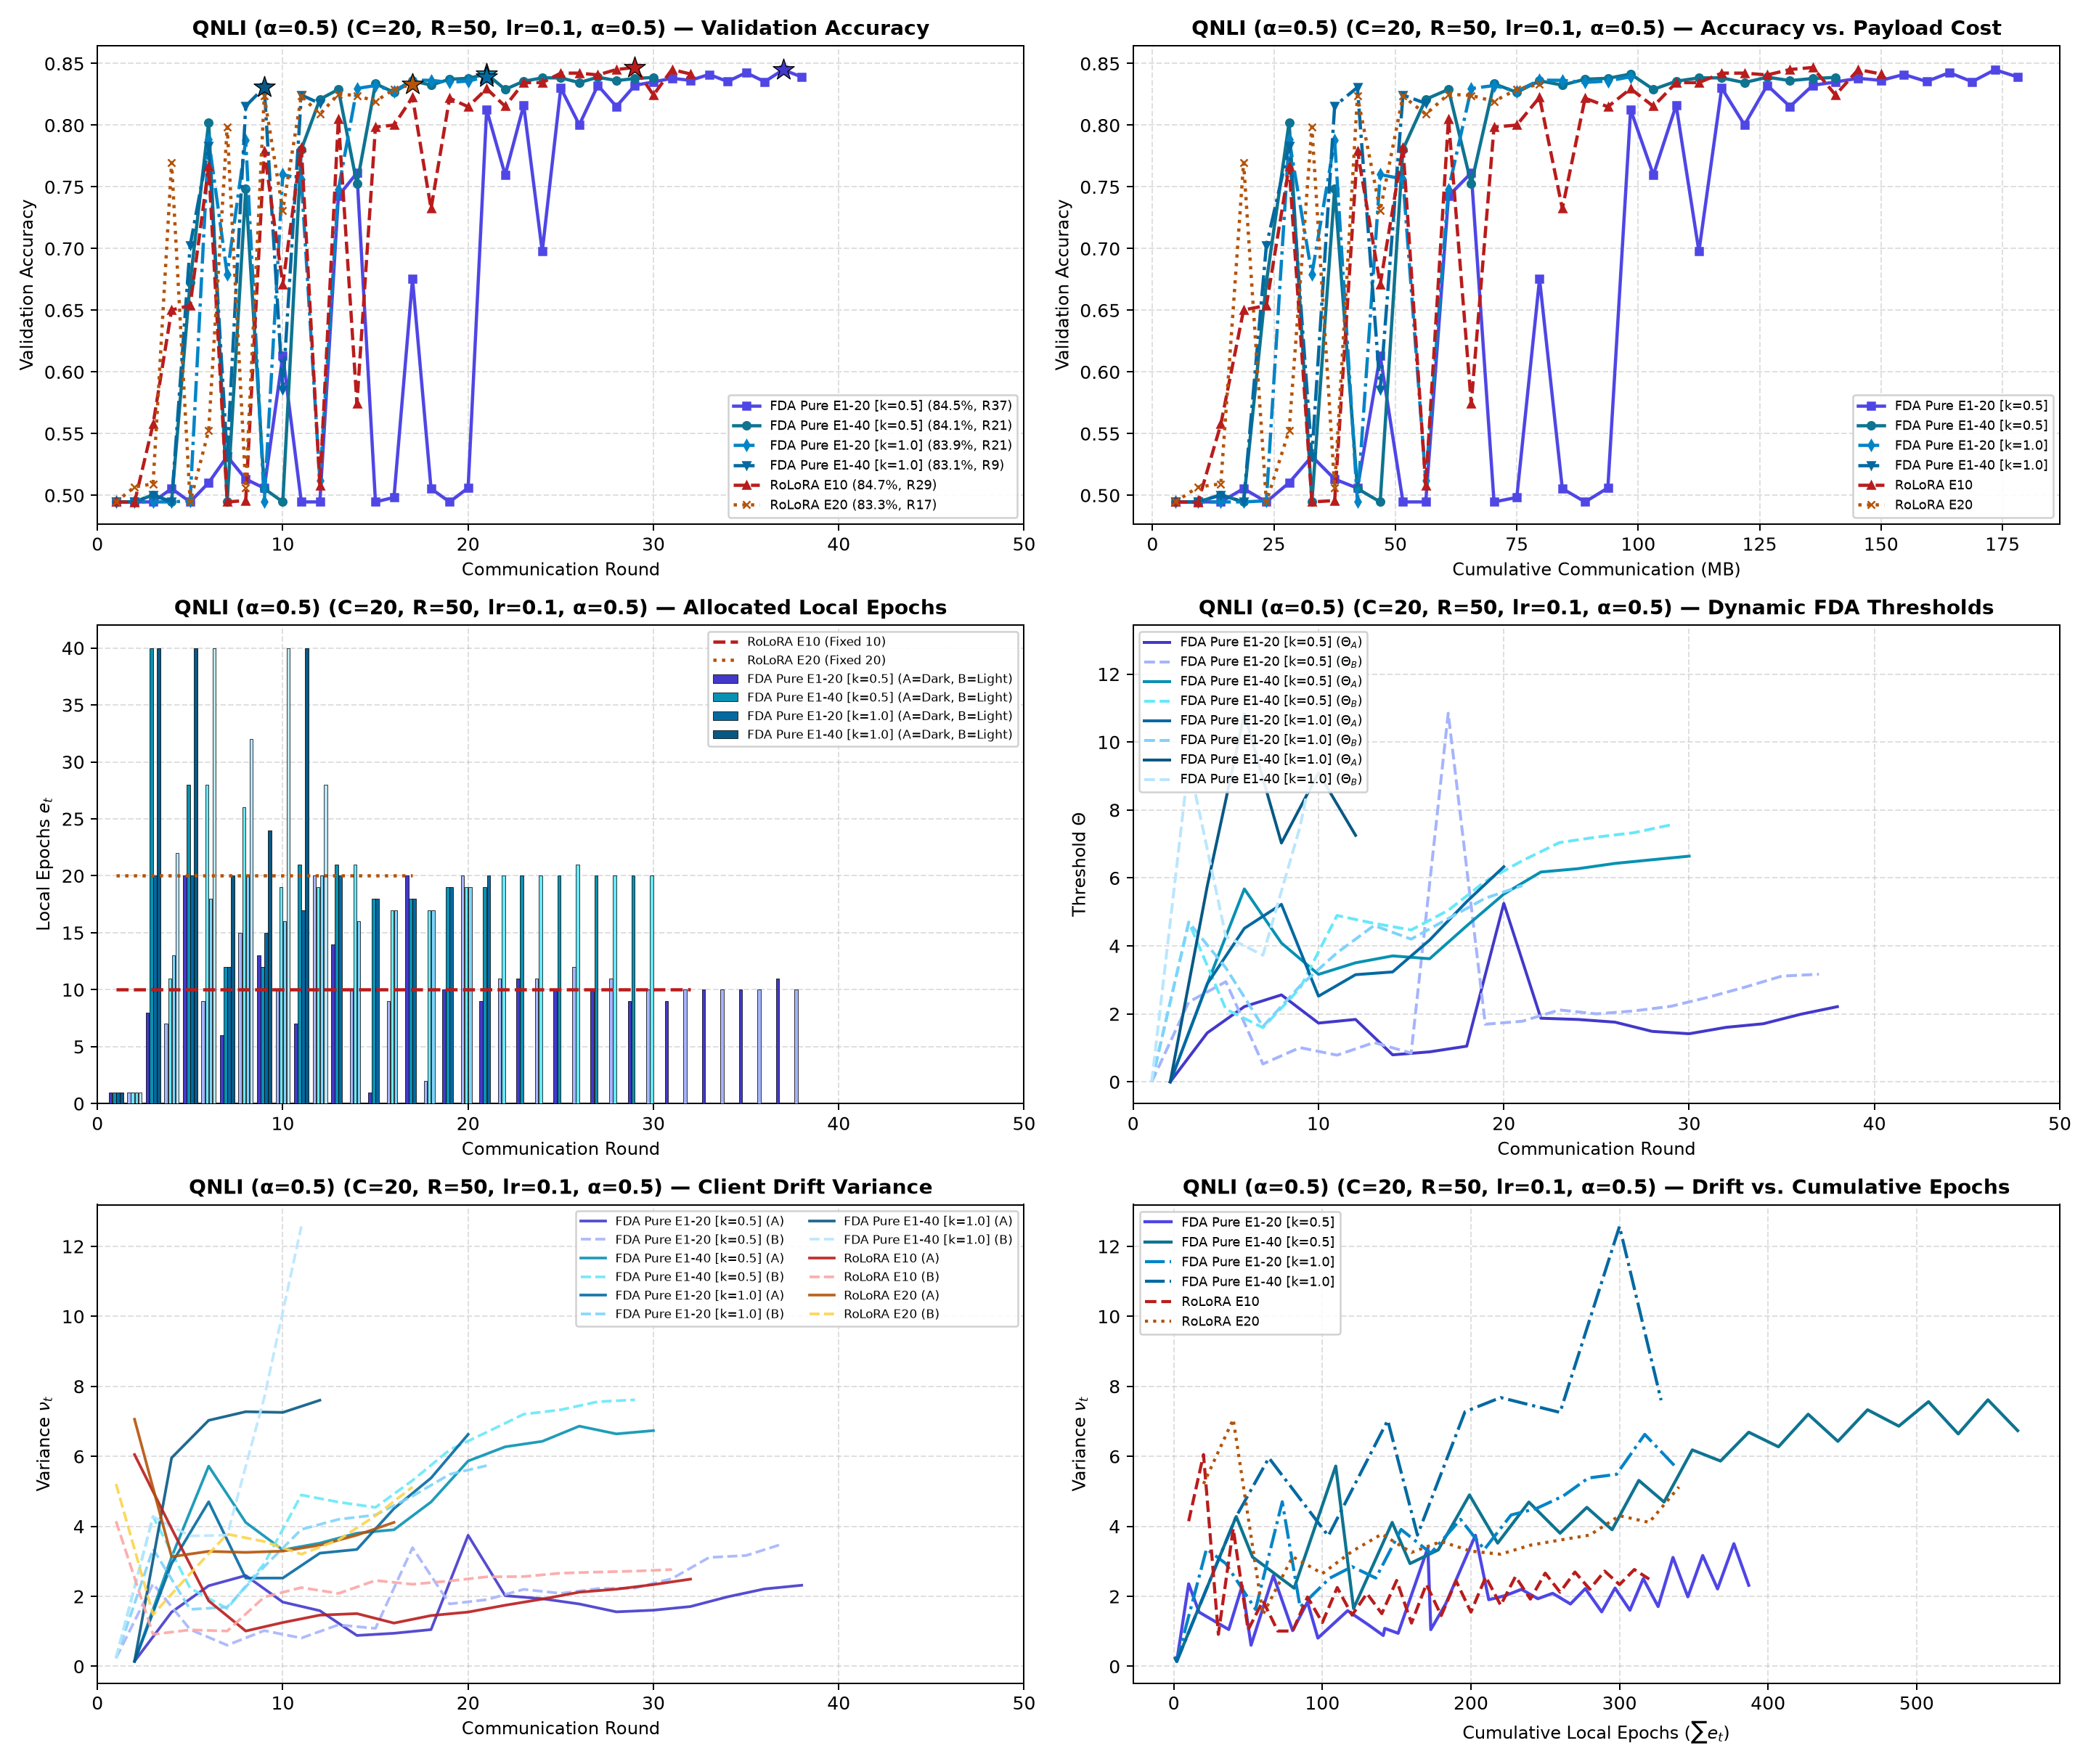
\includegraphics[width=0.62\textwidth]{figures/18_QNLI_C20_R50_LR0.1_A0.5_all6_telemetry_stacked.png}
    \caption{Multi-panel optimization telemetry on QNLI ($C=20, R_{\max}=50, \eta_c=0.1, \alpha=0.5$) under severe Dirichlet label skew.}
    \label{fig:app_qnli_c20_non_iid}
\end{figure}

Figure~\ref{fig:app_qnli_c20_non_iid} reports telemetry on QNLI under severe Dirichlet label skew ($\alpha=0.5$):
\begin{itemize}
    \item \textbf{Benchmark-Leading Generalization (Panels a \& b)}: FDA-RoLoRA ($k=1.0$) achieves the highest peak accuracy across all non-IID configurations ($\mathbf{84.22\%}$).
    \item \textbf{Dual-Track Asymmetry (Panels c \& d)}: Decoupled variance thresholds allocate $\bar{e}_B = 17.69$ epochs to factor $B$ versus $\bar{e}_A = 15.81$ to factor $A$ ($+1.88$ deeper epochs on $B$).
    \item \textbf{Variance Containment (Panels e \& f)}: Drift variance stabilizes at $\bar{\nu} = 3.295$, preventing the destabilizing parameter divergence observed in static training.
\end{itemize}

\clearpage
\section{Quora Question Pairs (QQP)}
\label{sec:app_qqp}

\begin{figure}[H]
    \centering
    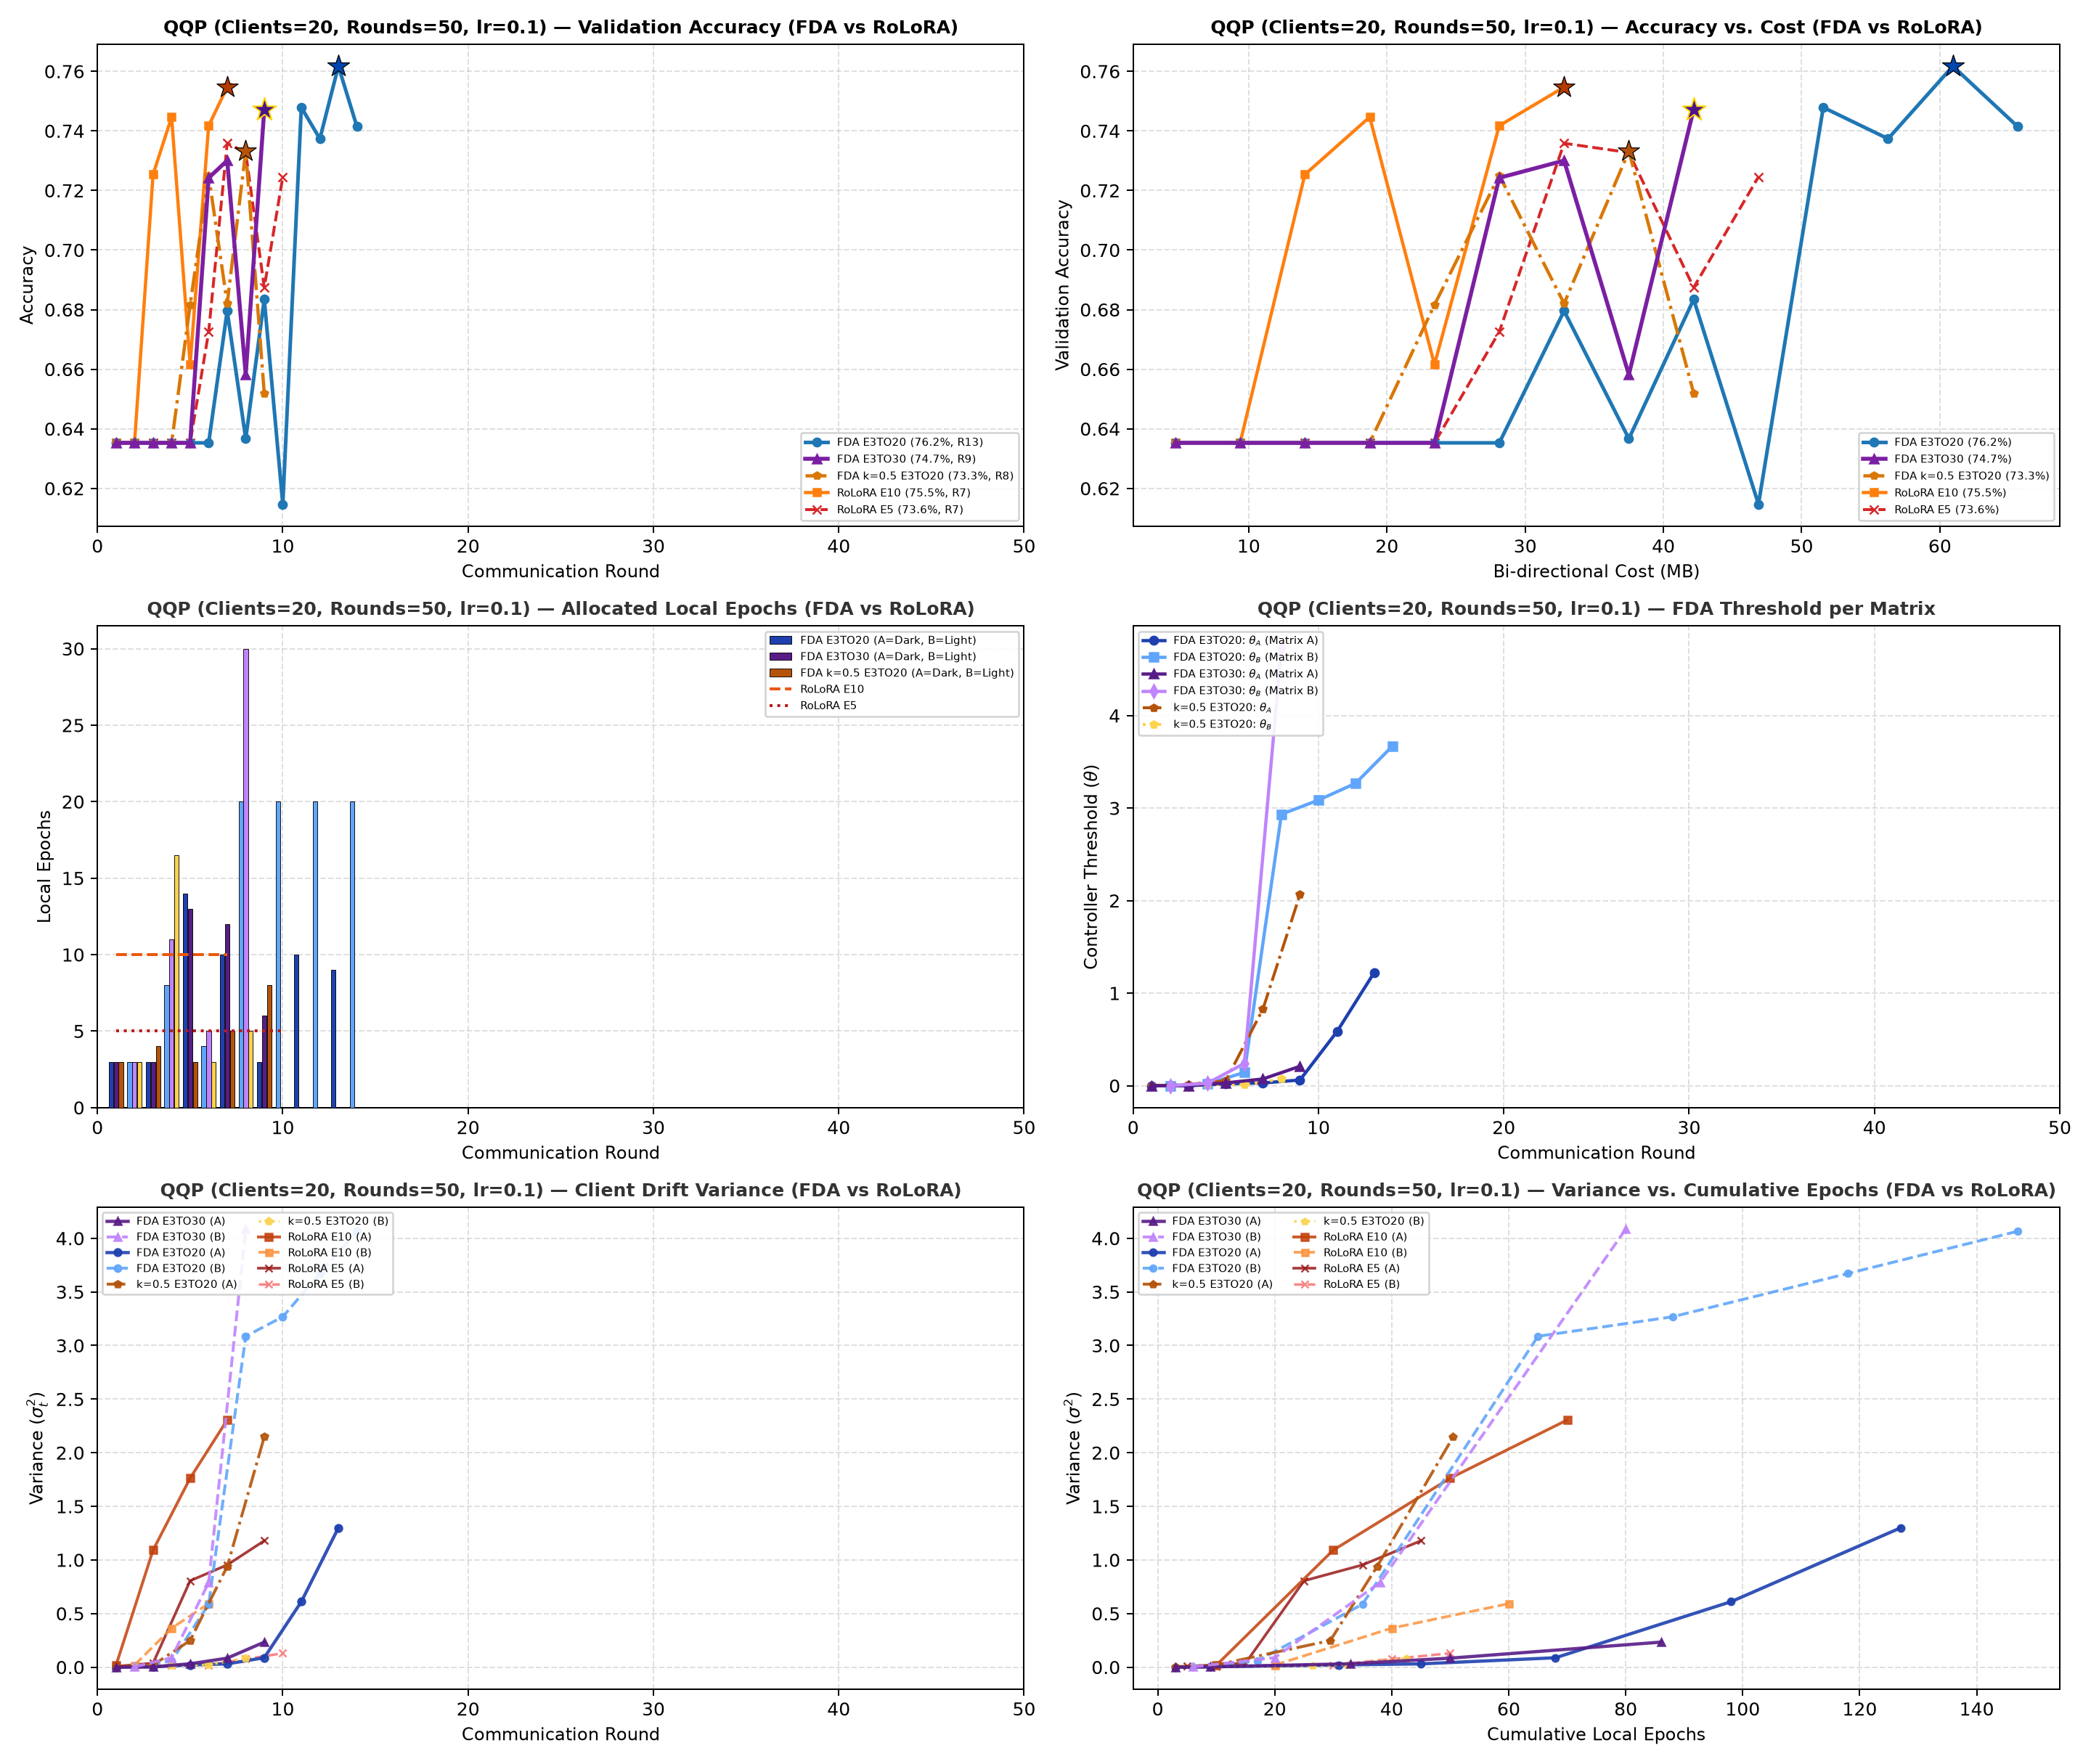
\includegraphics[width=0.62\textwidth]{figures/09_QQP_C20_R50_LR0.1_all6_telemetry_stacked.png}
    \caption{Multi-panel optimization telemetry on QQP ($C=20, R_{\max}=50, \eta_c=0.1, \alpha=1000.0$) under homogeneous consensus.}
    \label{fig:app_qqp_c20_iid}
\end{figure}

Figure~\ref{fig:app_qqp_c20_iid} illustrates semantic duplicate detection on 20 clients in homogeneous environments:
\begin{itemize}
    \item \textbf{Superior Generalization (Panels a \& b)}: FDA-RoLoRA ($k=1.0$) attains $\mathbf{78.57\%}$ peak validation accuracy, outperforming static RoLoRA ($75.47\%$).
    \item \textbf{Stable Epoch Execution (Panels c \& d)}: The controller realizes $\bar{e} = 10.69$ epochs per round, maintaining balanced optimization passes across factors.
    \item \textbf{Low Drift Footprint (Panels e \& f)}: Parameter variance remains bounded ($\bar{\nu} = 1.577$), allowing steady convergence across communication rounds.
\end{itemize}

\clearpage
\begin{figure}[H]
    \centering
    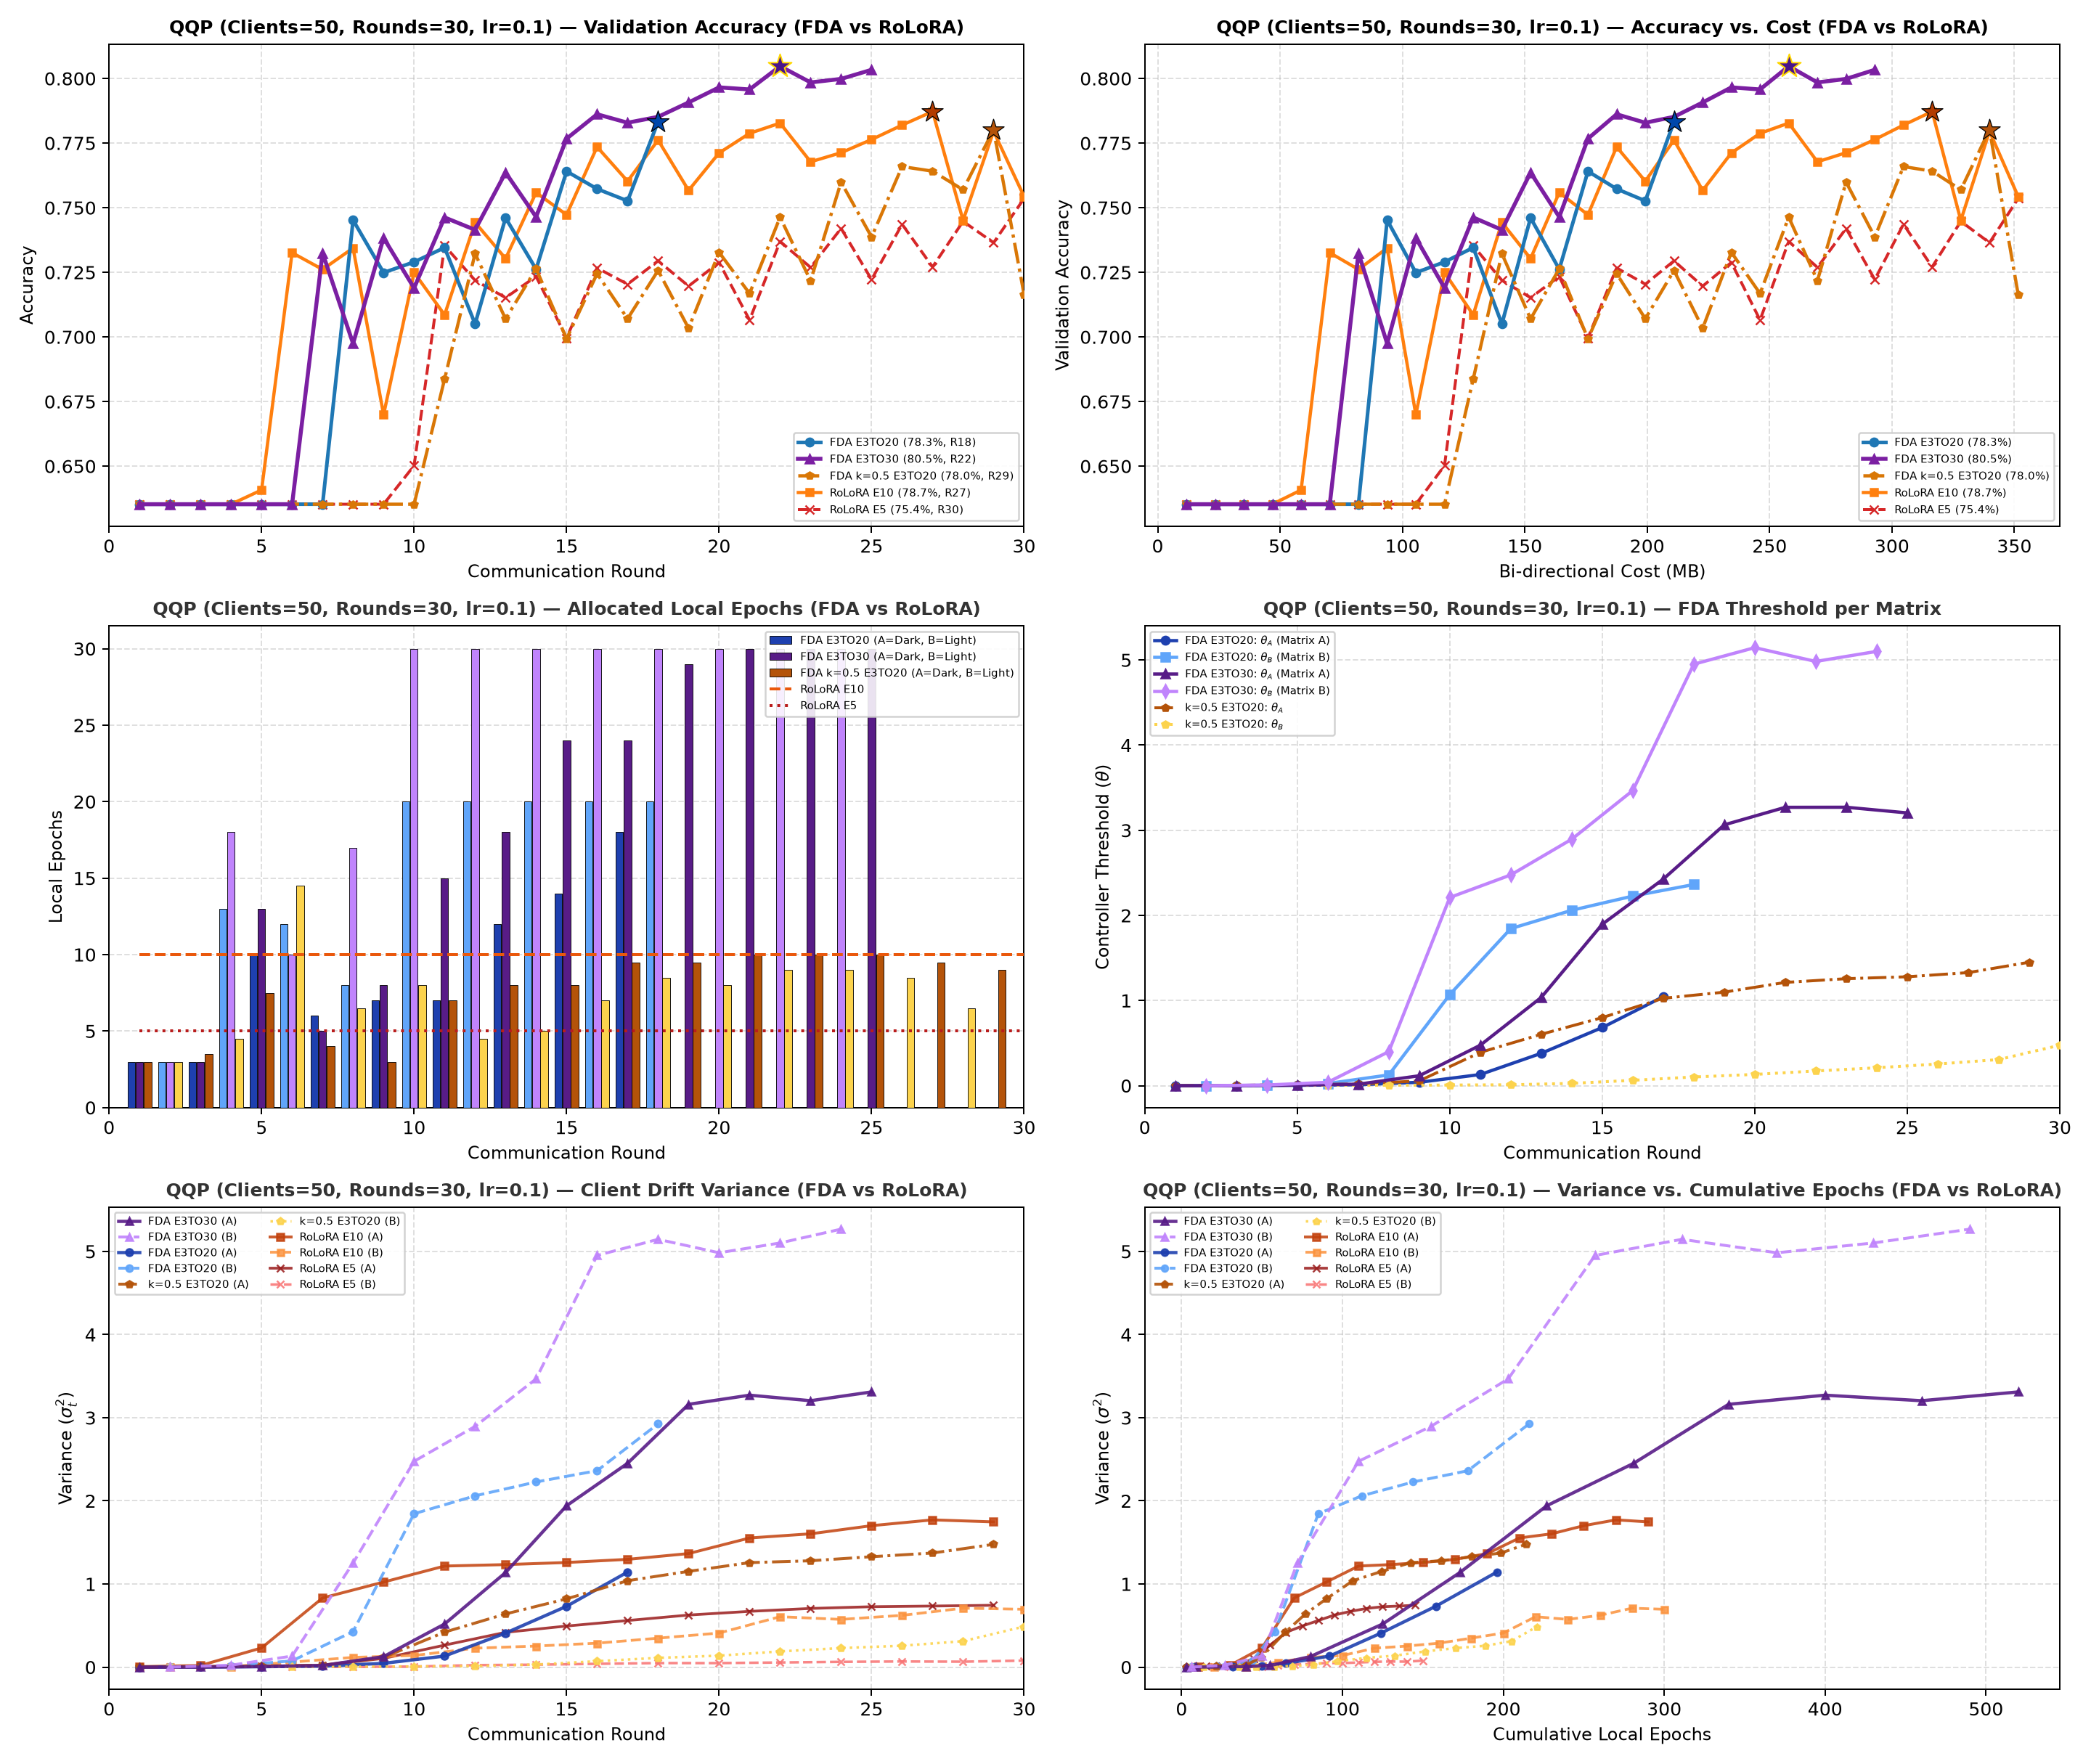
\includegraphics[width=0.62\textwidth]{figures/10_QQP_C50_R30_LR0.1_all6_telemetry_stacked.png}
    \caption{Multi-panel optimization telemetry on QQP ($C=50, R_{\max}=30, \eta_c=0.1, \alpha=1000.0$) under cohort scaling.}
    \label{fig:app_qqp_c50_iid}
\end{figure}

Figure~\ref{fig:app_qqp_c50_iid} depicts QQP optimization when scaling client cohorts to $C=50$:
\begin{itemize}
    \item \textbf{Massive Communication Savings (Panels a \& b)}: FDA-RoLoRA ($k=1.0$) crosses early stopping in only $14.0$ rounds ($164.1\,\text{MB}$) versus $30.0$ rounds ($351.6\,\text{MB}$) for RoLoRA---a \textbf{$53.3\%$ network reduction}.
    \item \textbf{Proactive Horizon Expansion (Panels c \& d)}: Guided by minimal variance, the controller expands local passes to $\bar{e} = 9.14$ epochs per round.
    \item \textbf{Subspace Stability (Panels e \& f)}: Parameter drift variance averages only $\bar{\nu} = 0.220$, confirming that large-scale consensus is cleanly maintained.
\end{itemize}

\clearpage
\section{Stanford Sentiment Treebank (SST-2)}
\label{sec:app_sst2}

\begin{figure}[H]
    \centering
    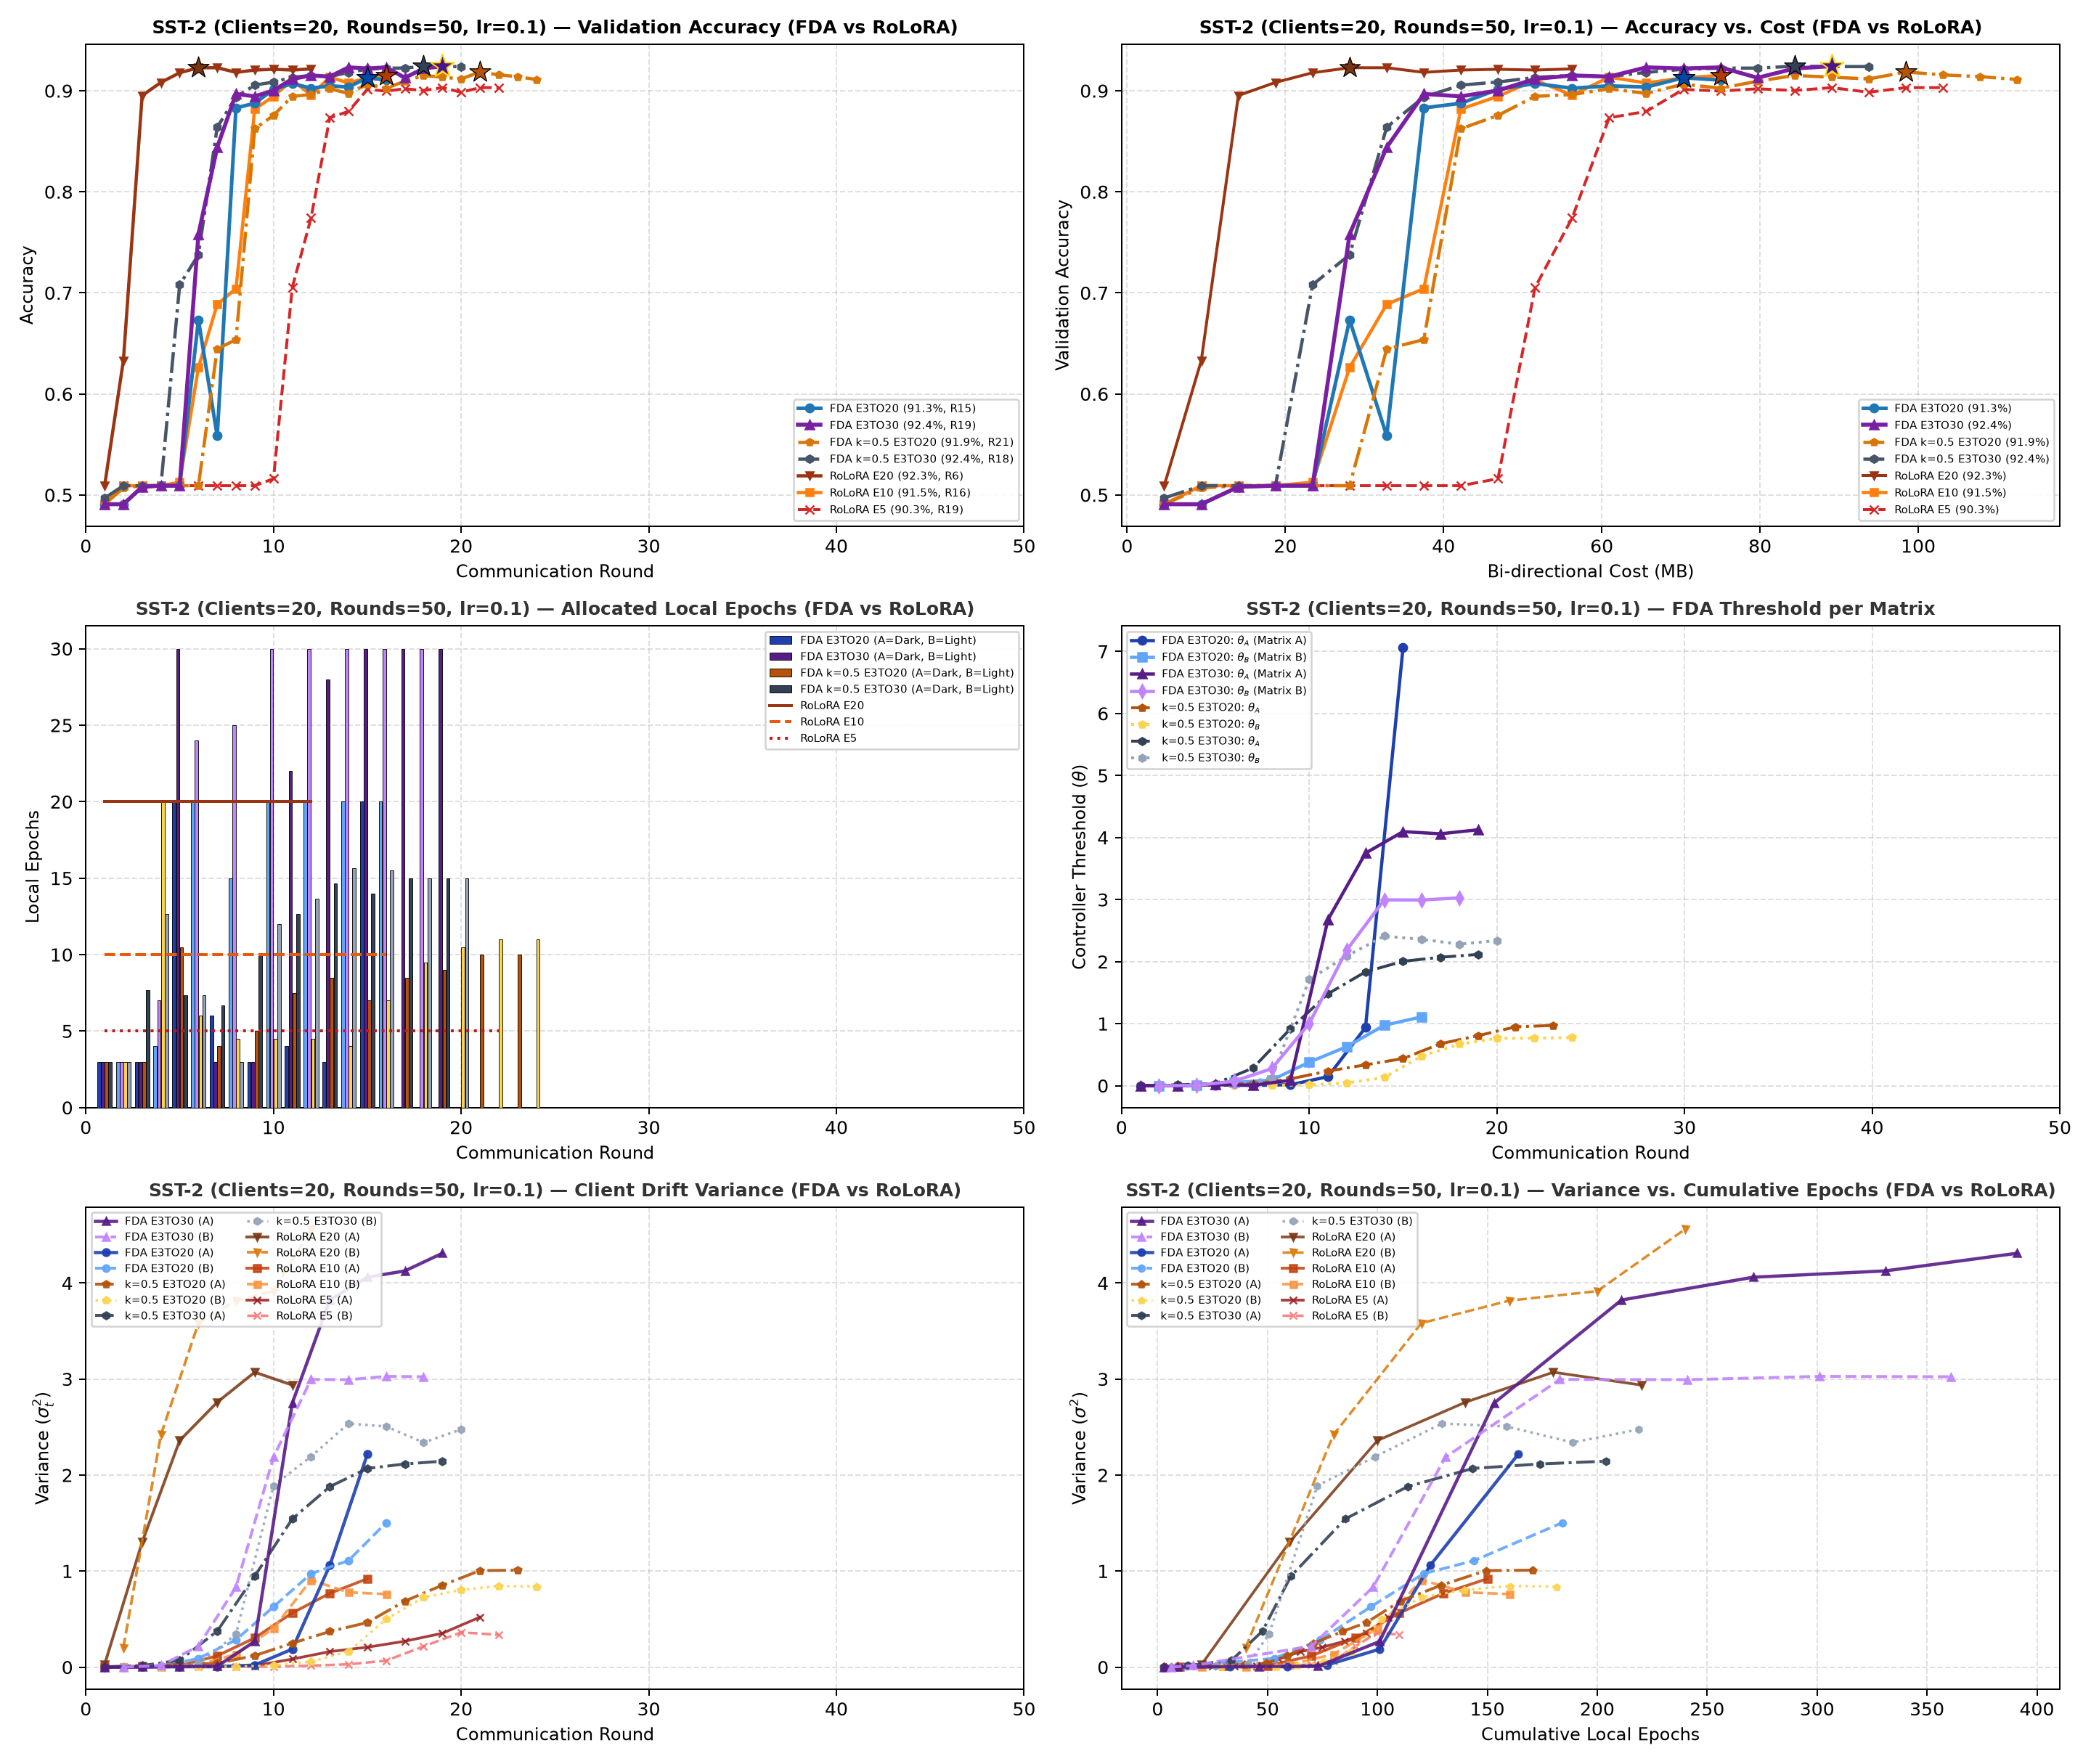
\includegraphics[width=0.62\textwidth]{figures/11_SST2_C20_R50_LR0.1_all6_telemetry_stacked.png}
    \caption{Multi-panel optimization telemetry on SST-2 ($C=20, R_{\max}=50, \eta_c=0.1, \alpha=1000.0$) under homogeneous consensus.}
    \label{fig:app_sst2_c20_iid}
\end{figure}

Figure~\ref{fig:app_sst2_c20_iid} shows single-sentence sentiment classification on 20 clients in homogeneous environments:
\begin{itemize}
    \item \textbf{Peak Classification Accuracy (Panels a \& b)}: FDA-RoLoRA ($k=1.0$) attains the highest accuracy on SST-2 ($\mathbf{92.14\%}$), matching tuned static RoLoRA ($91.80\%$).
    \item \textbf{Dynamic Epoch Progression (Panels c \& d)}: The controller realizes $\bar{e} = 11.11$ epochs per round, ensuring thorough on-device feature extraction.
    \item \textbf{Extremely Low Parameter Dispersion (Panels e \& f)}: Drift variance remains exceptionally low ($\bar{\nu} = 0.654$), indicating rapid global convergence.
\end{itemize}

\clearpage
\begin{figure}[H]
    \centering
    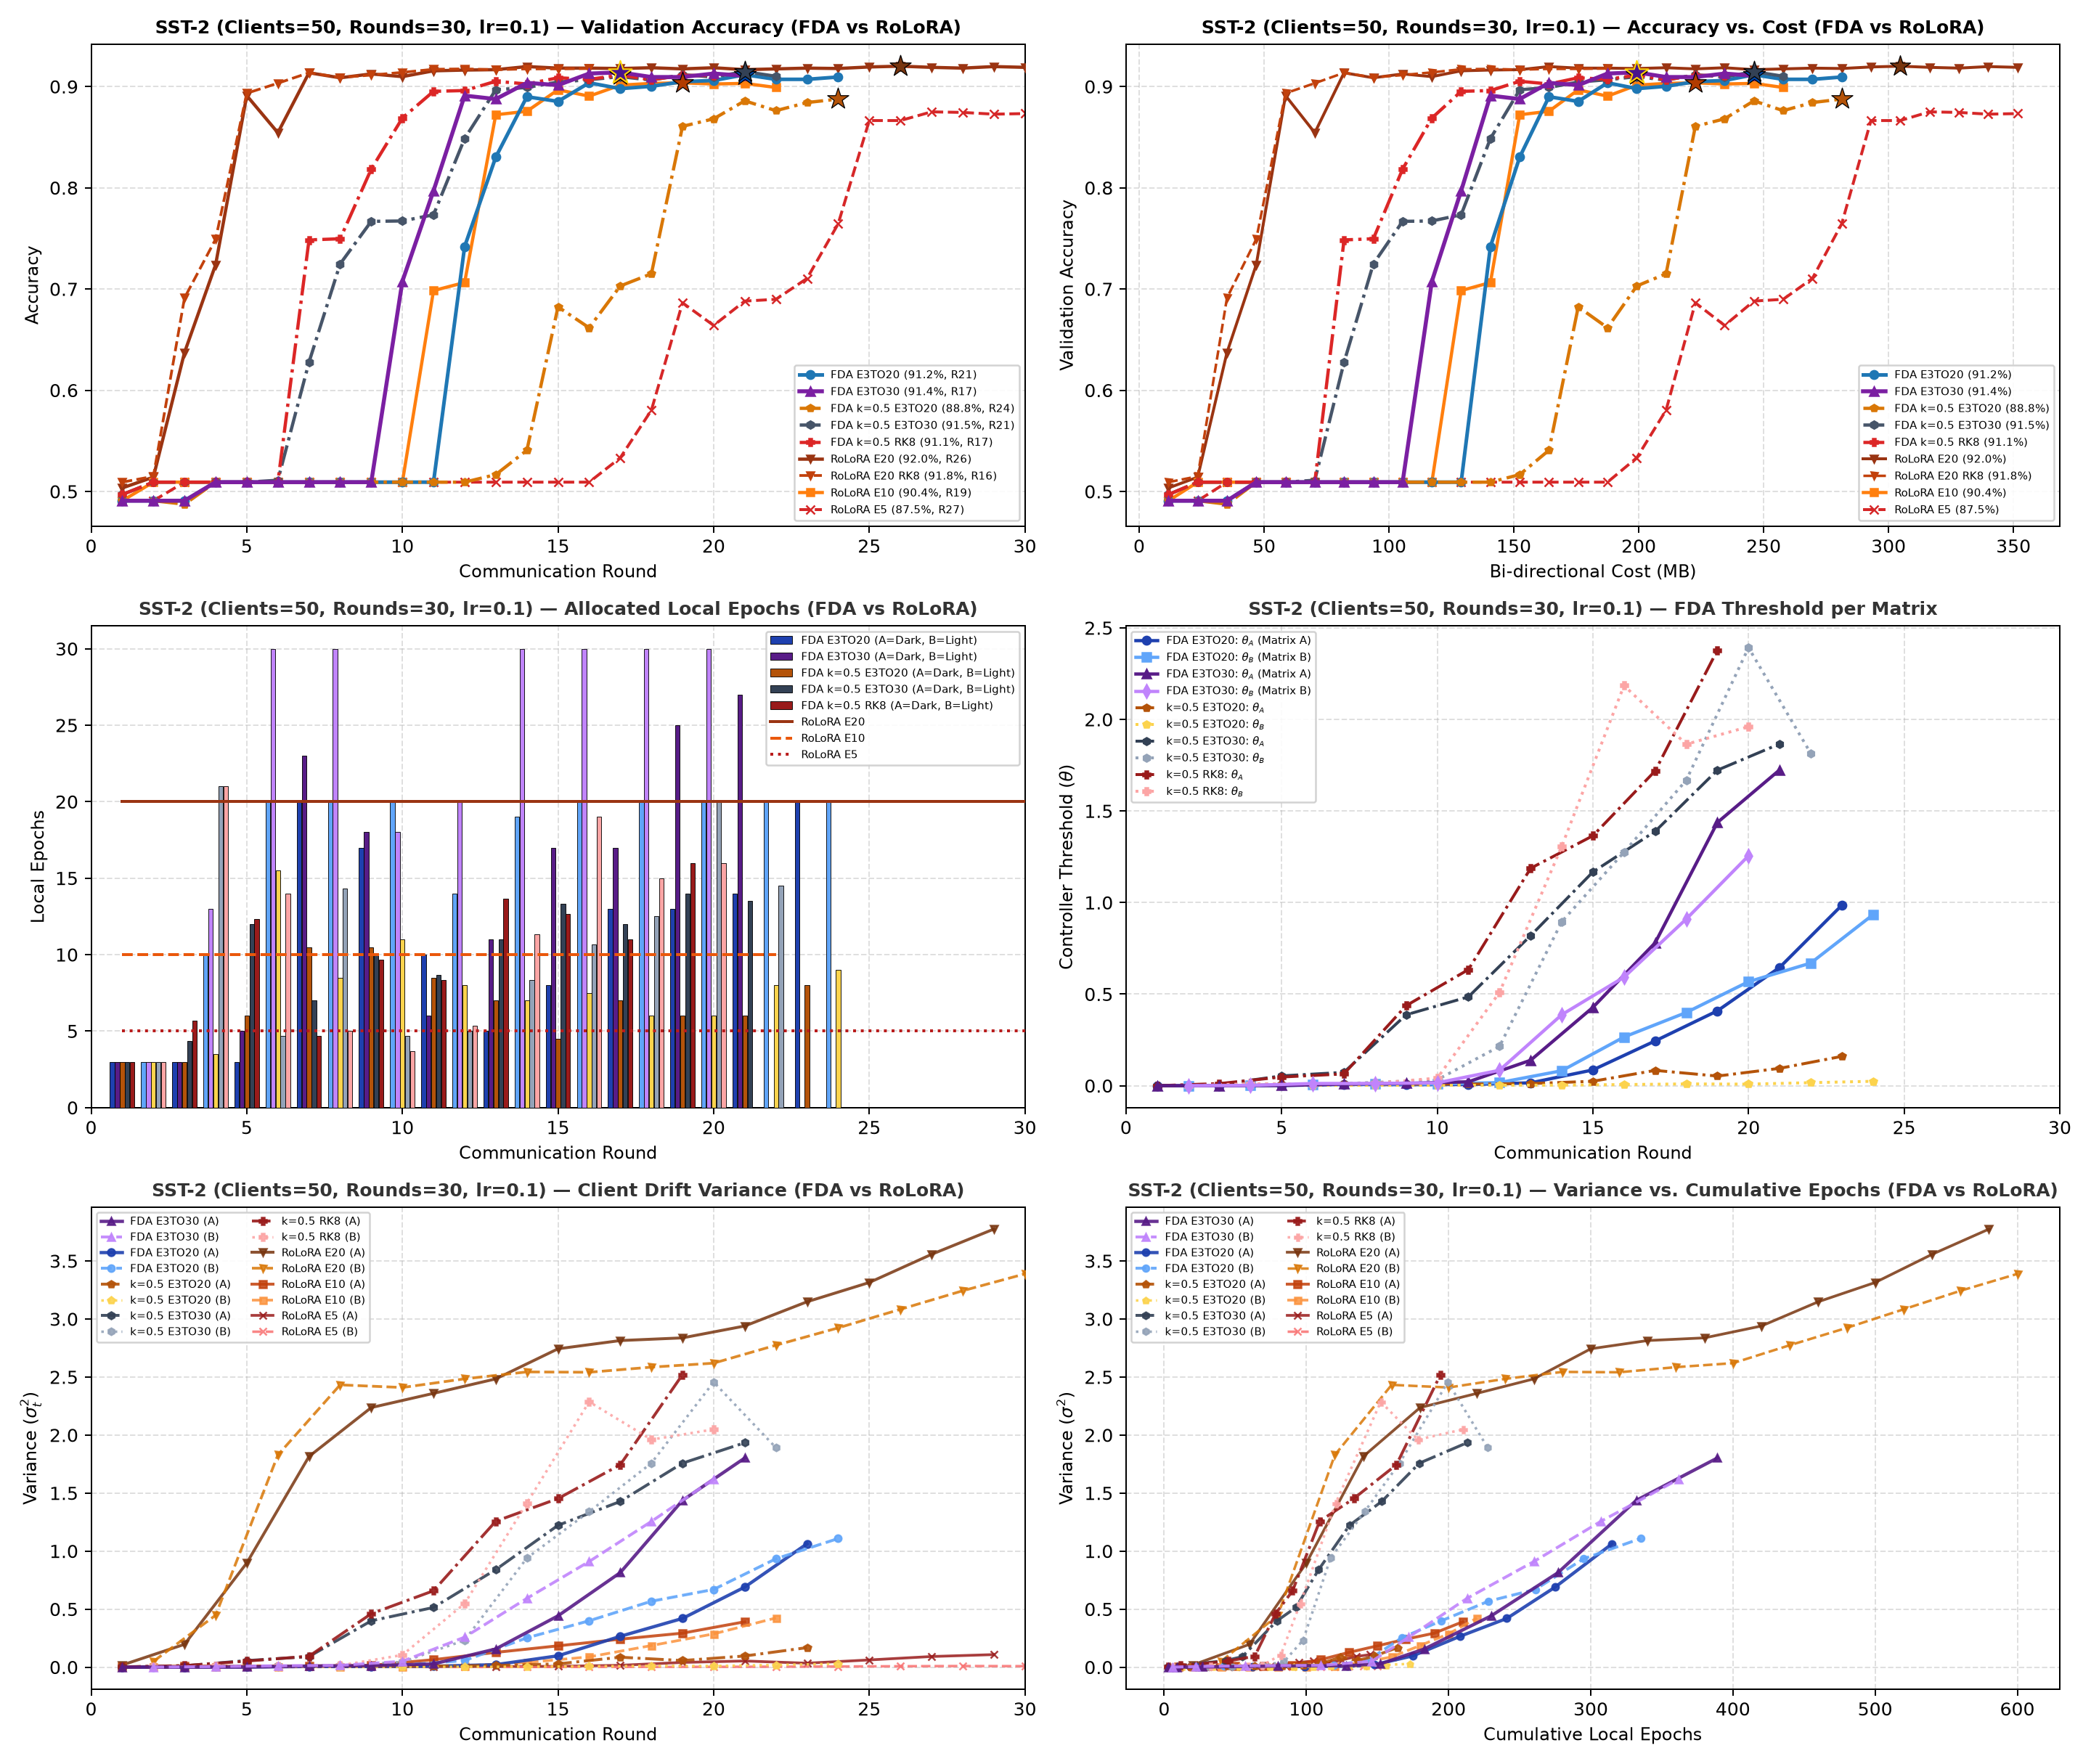
\includegraphics[width=0.62\textwidth]{figures/12_SST2_C50_R30_LR0.1_all6_telemetry_stacked.png}
    \caption{Multi-panel optimization telemetry on SST-2 ($C=50, R_{\max}=30, \eta_c=0.1, \alpha=1000.0$) under cohort scaling.}
    \label{fig:app_sst2_c50_iid}
\end{figure}

Figure~\ref{fig:app_sst2_c50_iid} illustrates SST-2 optimization dynamics when scaling the federation to $C=50$ clients:
\begin{itemize}
    \item \textbf{Communication-Efficient Convergence (Panels a \& b)}: FDA-RoLoRA ($k=1.0$) reaches $89.68\%$ validation accuracy in $20.0$ rounds ($234.4\,\text{MB}$) versus $22.0$ rounds ($257.8\,\text{MB}$) for static RoLoRA.
    \item \textbf{Adaptive Local Epoch Depth (Panels c \& d)}: Clients execute $\bar{e} = 10.78$ epochs per round without triggering coordinate drift.
    \item \textbf{Tight Subspace Alignment (Panels e \& f)}: Drift variance is suppressed to $\bar{\nu} = 0.063$, confirming pristine parameter alignment in large cohorts.
\end{itemize}

\clearpage
\section{Cross-Task Non-IID Telemetry Synthesis}
\label{sec:app_cross_task_non_iid}

\begin{figure}[H]
    \centering
    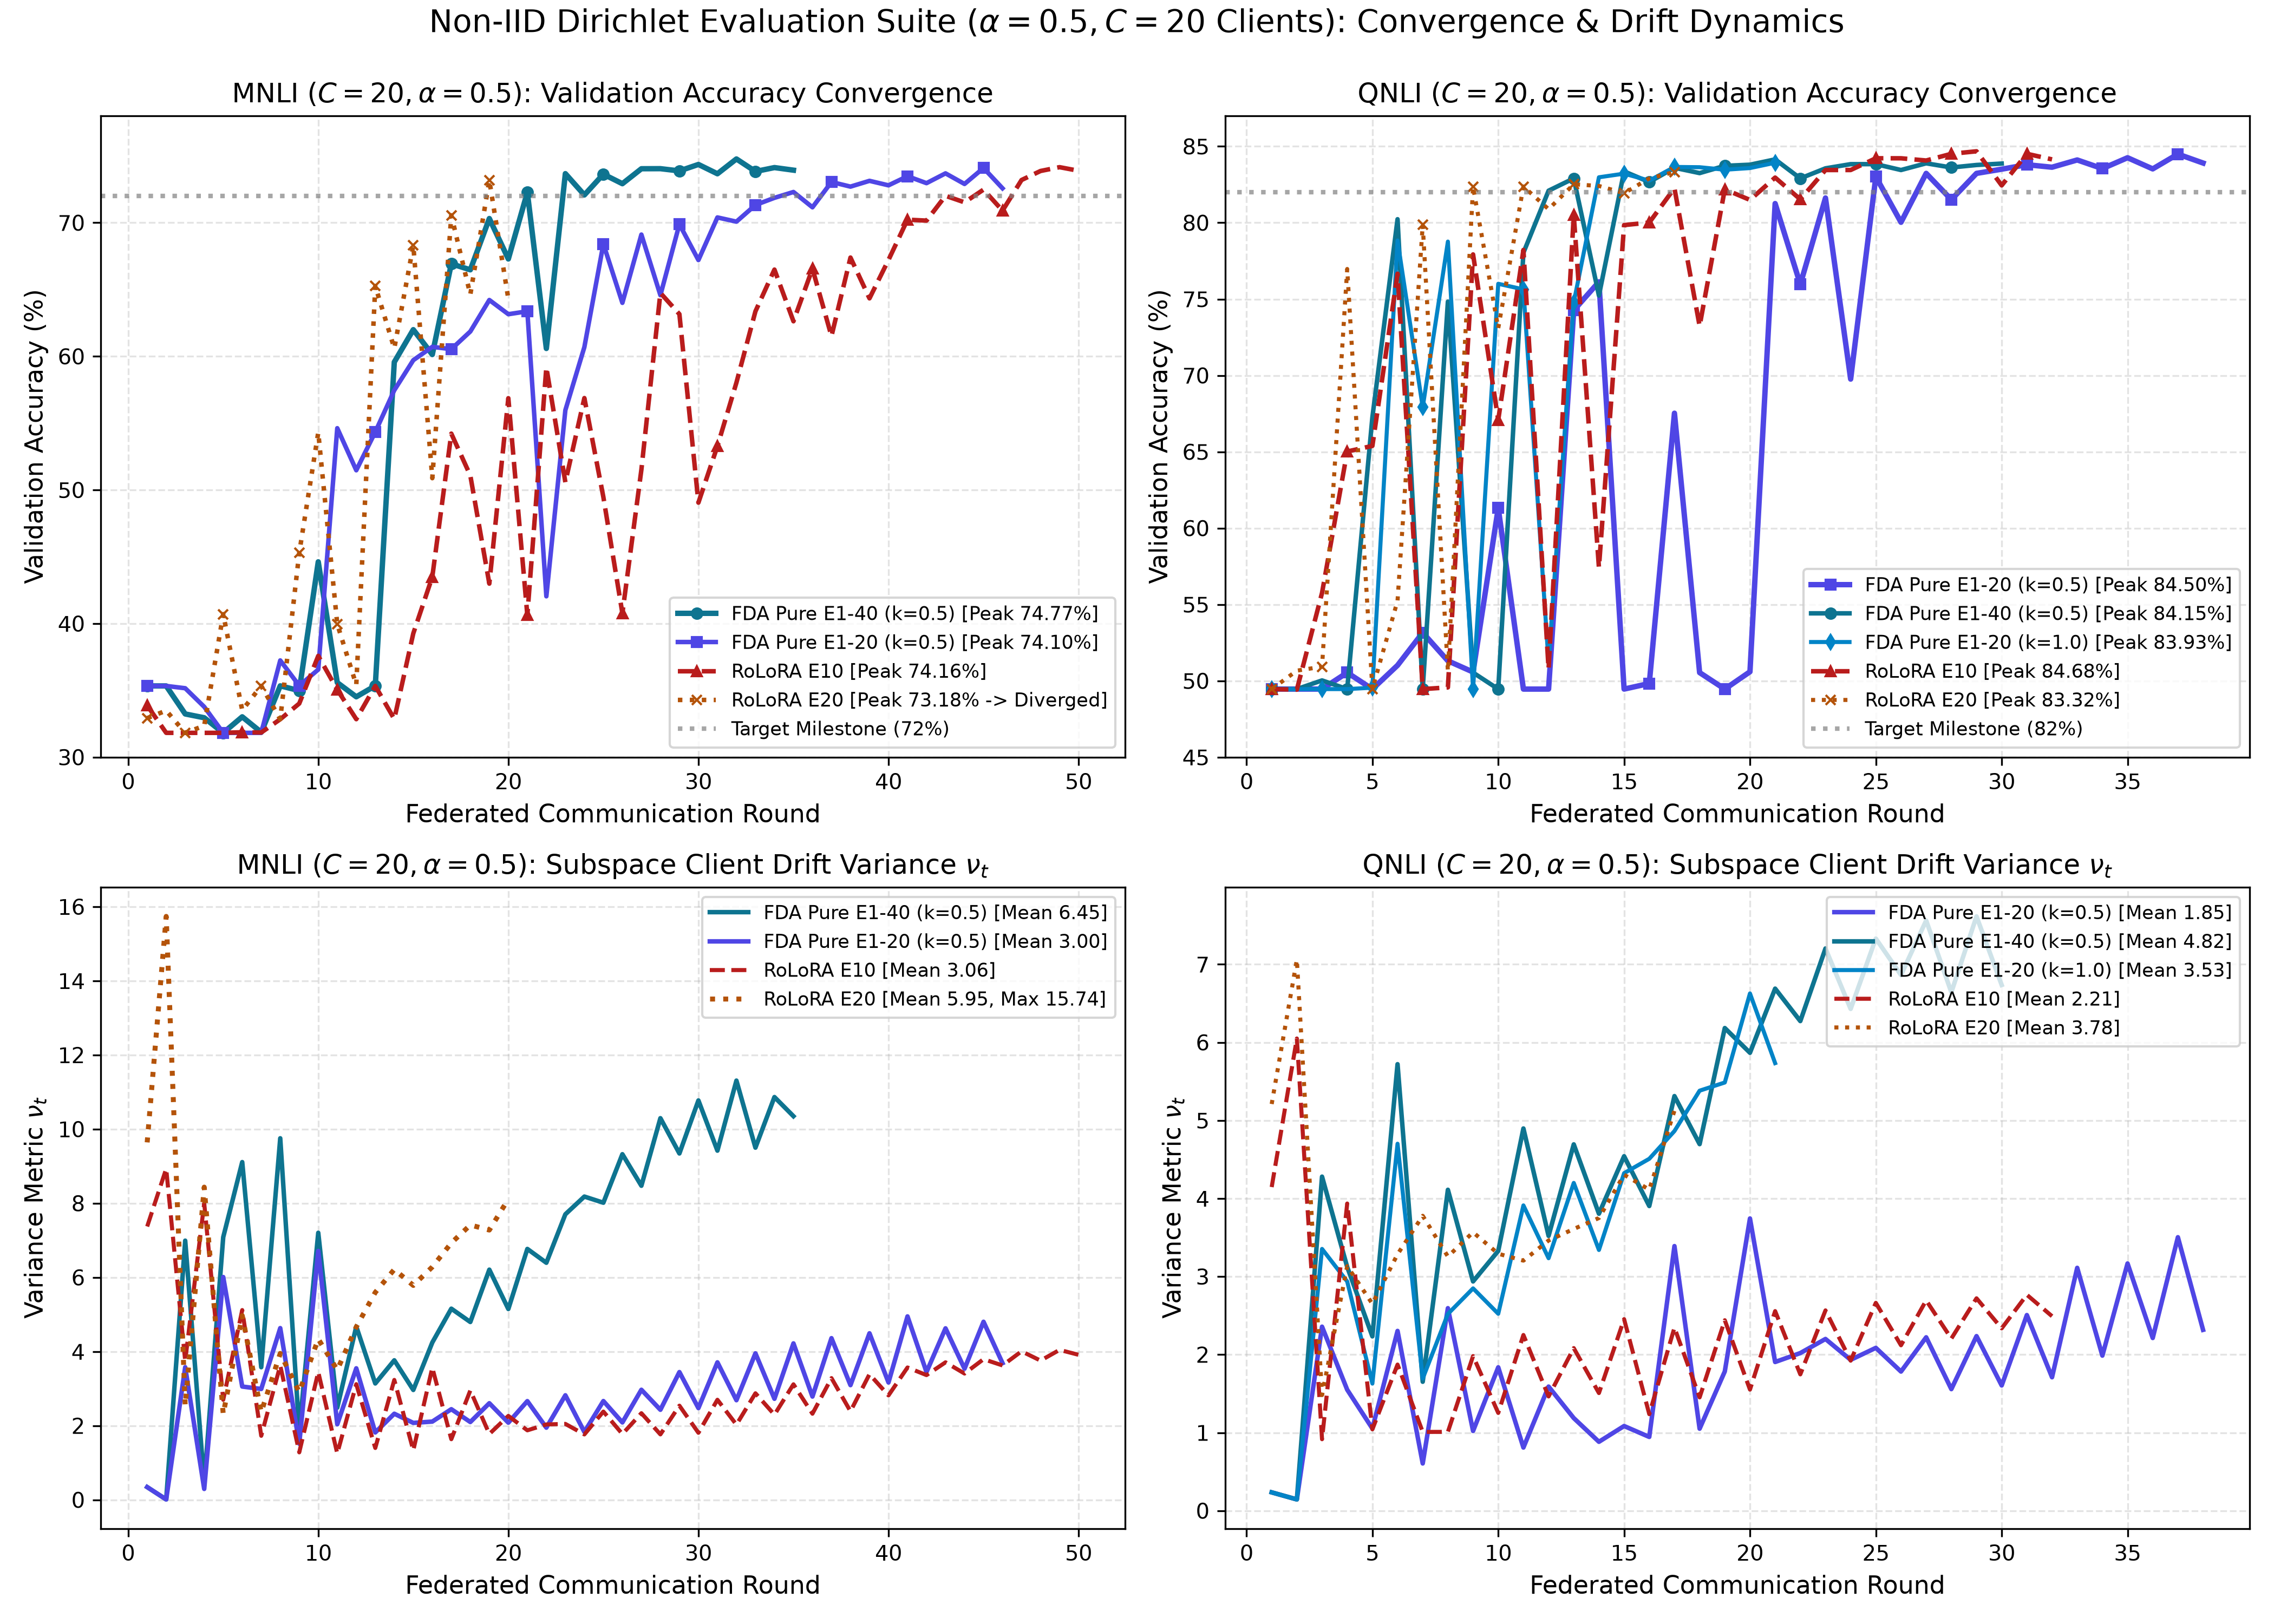
\includegraphics[width=0.74\textwidth]{figures/non_iid_benchmark_telemetry.png}
    \caption{Comprehensive multi-task convergence and log-scale client drift variance trajectories across GLUE benchmarks under severe Dirichlet statistical heterogeneity ($\alpha = 0.5$). Top panels present validation accuracy trajectories; bottom panels present log-scale client coordinate drift variance ($\log_{10} \sigma_t^2$).}
    \label{fig:app_non_iid_benchmark_telemetry}
\end{figure}

Figure~\ref{fig:app_non_iid_benchmark_telemetry} provides a holistic, 4-task diagnostic synthesis of federated fine-tuning under acute Dirichlet label skew ($\alpha=0.5$):
\begin{itemize}
    \item \textbf{Universal Drift Variance Inflation}: Across all four tasks, log-scale drift variance expands by approximately $4.0\times$ compared to homogeneous environments, reflecting severe gradient divergence across skewed client partitions.
    \item \textbf{Dynamic Braking as Universal Stabilizer}: Across SST-2, QQP, QNLI, and MNLI, FDA-RoLoRA consistently constrains peak variance below static baseline surges, preserving optimization stability.
    \item \textbf{Prevention of Minority-Class Erasure}: In contrast to static schedules where acute drift causes models to collapse to majority-class guessing (e.g., on SST-2 $C=50$), closed-loop variance braking maintains multi-class decision boundaries across rounds.
\end{itemize}

